\documentclass{article}
\usepackage{amsthm,hyperref,mathtools,mathpartir,cleveref,mathrsfs,amssymb,url,paralist,xspace,braket,ifmtarg,cancel}
\usepackage[status=draft,author=]{fixme}
\fxusetheme{color}
\newtheorem{thm}{Theorem}[section]
\crefname{thm}{Theorem}{Theorems}
\newtheorem{lem}[thm]{Lemma}
\crefname{lem}{Lemma}{Lemmas}
\newtheorem{cor}[thm]{Corollary}
\crefname{cor}{Corollary}{Corollaries}
\newtheorem{conj}[thm]{Corollary}
\crefname{conj}{Conjecture}{Conjectures}
\theoremstyle{definition}
\newtheorem{defn}[thm]{Definition}
\crefname{defn}{Definition}{Definitions}
\newtheorem{defns}[thm]{Definitions}
\crefname{defns}{Definitions}{Definitions}
\newtheorem{eg}[thm]{Example}
\crefname{eg}{Example}{Examples}
\theoremstyle{remark}
\newtheorem{rmk}[thm]{Remark}
\crefname{rmk}{Remark}{Remarks}
\usepackage{tikz}
\usepackage{tikz-cd}
\usetikzlibrary{decorations.markings}
\tikzset{edge/.style={decoration={markings,mark=at position 0.5 with {\arrow{>}}},postaction={decorate}}}
\tikzset{vertex/.style={circle,draw,inner sep=1pt}}
\usetikzlibrary{shapes.geometric}
\tikzset{outer/.style={regular polygon,regular polygon sides=3,inner sep=1pt,draw,shape border rotate=180}}
\tikzset{houter/.style={regular polygon,regular polygon sides=3,inner sep=1pt,draw,shape border rotate=270}}
\tikzset{cross/.style={white,line width=3pt}}
\let\sto\looparrowright
\def\M{\mathbb{M}}
\def\A{\mathcal{A}}
\def\B{\mathcal{B}}
\def\C{\mathcal{C}}
\def\P{\mathcal{P}}
\def\Q{\mathcal{Q}}
\def\D{\mathcal{D}}
\def\G{\mathcal{G}}
\def\H{\mathcal{H}}
\def\K{\mathbb{K}}
\def\L{\mathcal{L}}
\def\R{\mathcal{R}}
\def\V{\mathscr{V}}
\def\frob{\mathbb{F}\mathsf{rob}}
\def\ten{\mathbb{T}\mathsf{en}}
\def\hspan{\mathbb{HS}\mathsf{pan}}
\def\form#1{\mathsf{F}_{#1}}
\let\setof\Set
\def\Set{\mathbf{Set}}
\def\Cat{\ensuremath{\mathcal{C}\mathit{at}}}
%\def\Cat{\ensuremath{\mathbf{Cat}}}
\def\Fib{\mathcal{F}\mathit{ib}}
\def\SFib{\mathcal{SF}\mathit{ib}}
\def\Prof{\mathcal{P}\mathit{rof}}
\def\cpg{\ensuremath{\mathcal{CPG}}\xspace}
\def\dom{\mathrm{dom}}
\def\cod{\mathrm{cod}}
\def\id{\mathrm{id}}
\def\Id{\mathrm{Id}}
\def\side#1{{\scriptstyle(#1)}}
\def\sid{\side{\id}}
% \def\twocell#1#2#3#4{\inferrule*[Left={$\side{#1}$},Right={$\side{#4}$}]{#2}{#3}}
% \def\twocelll#1#2#3#4{\inferrule*[left={$\side{#1}$},Right={$\side{#4}$}]{#2}{#3}}
% \def\twocellr#1#2#3#4{\inferrule*[Left={$\side{#1}$},right={$\side{#4}$}]{#2}{#3}}
% \def\twocelllr#1#2#3#4{\inferrule*[left={$\side{#1}$},right={$\side{#4}$}]{#2}{#3}}

\def\op{^{\mathrm{op}}}
\def\lan{\operatorname{Lan}}

\newcounter{nodemaker}
\setcounter{nodemaker}{0}
\newcommand{\twocell}[2][]{%
  \global\edef\mynodeone{twocell\arabic{nodemaker}}%
  \stepcounter{nodemaker}%
  \global\edef\mynodetwo{twocell\arabic{nodemaker}}%
  \stepcounter{nodemaker}%
  \ar[#2,phantom,shift left=3,""{name=\mynodeone}]%
  \ar[#2,phantom,shift right=3,""'{name=\mynodetwo}]%
  \ar[Rightarrow,from=\mynodeone,to=\mynodetwo,"{#1}"]%
}
\newcommand{\twocellop}[2][]{%
  \global\edef\mynodeone{twocell\arabic{nodemaker}}%
  \stepcounter{nodemaker}%
  \global\edef\mynodetwo{twocell\arabic{nodemaker}}%
  \stepcounter{nodemaker}%
  \ar[#2,phantom,shift left=3,""{name=\mynodeone}]%
  \ar[#2,phantom,shift right=3,""'{name=\mynodetwo}]%
  \ar[Rightarrow,from=\mynodetwo,to=\mynodeone,"{#1}"]%
}
\newcommand{\drpullback}[1][dr]{\ar[#1,phantom,near start,"\lrcorner"]}
\newcommand{\dlpullback}[1][dl]{\ar[#1,phantom,near start,"\llcorner"]}
\newcommand{\urpullback}[1][ur]{\ar[#1,phantom,near start,"\urcorner"]}
\newcommand{\ulpullback}[1][ul]{\ar[#1,phantom,near start,"\ulcorner"]}

\let\ot\leftarrow
\let\xto\xrightarrow
\let\xot\xleftarrow
\let\tot\leftrightarrow
\def\o{^{\circ}}
\tikzset{horiz/.style={"\mathclap\bullet" description}}
\def\genus{\mathsf{genus}}
\def\degree{\mathsf{degree}}
\def\rank{\mathsf{rank}}
\def\N{\mathbb{N}}
\def\Np{\N_{\bullet}}
% \def\hy{\mathcal{H}\mathit{y}\mathcal{G}\mathit{ph}}
\def\hyrel{\mathcal{H}\mathit{y}\mathcal{R}\mathit{el}}
\def\hy{\mathbf{HyGph}}
\def\RGph{\mathbf{RGph}}
\def\GCtx{\mathbf{GCtx}}
\def\hohy{\mathbf{HyGph}}
\def\thy{\mathcal{T}}
\def\dhy{\mathcal{D}}
\def\bhy{\mathcal{B}}
\def\fhy{\mathcal{F}}
\def\ehy{\mathcal{E}\mathit{xt}\mathcal{H}\mathit{y}\mathcal{G}\mathit{ph}}

% Get new symbols from mathabx without changing the old ones
\DeclareFontFamily{U}{mathb}{\hyphenchar\font45}
\DeclareFontShape{U}{mathb}{m}{n}{
      <5> <6> <7> <8> <9> <10> gen * mathb
      <10.95> mathb10 <12> <14.4> <17.28> <20.74> <24.88> mathb12
      }{}
\DeclareSymbolFont{mathb}{U}{mathb}{m}{n}
\DeclareFontSubstitution{U}{mathb}{m}{n}
%
\DeclareFontFamily{U}{mathx}{\hyphenchar\font45}
\DeclareFontShape{U}{mathx}{m}{n}{
      <5> <6> <7> <8> <9> <10>
      <10.95> <12> <14.4> <17.28> <20.74> <24.88>
      mathx10
      }{}
\DeclareSymbolFont{mathx}{U}{mathx}{m}{n}
\DeclareFontSubstitution{U}{mathx}{m}{n}
%
\DeclareMathSymbol{\Asterisk}{2}{mathb}{"06}
\DeclareMathSymbol{\bigboxtimes}{1}{mathx}{"D2}

\makeatletter
%\def\ins#1#2#3#4{#1 \underset{\@ifmtarg{#2}{#3}{#3\in #2}}{\circ} #4}
\def\ins#1#2#3#4{#1 \mathbin{{\Asterisk}_{\@ifmtarg{#2}{#3}{#3\in #2}}} #4}
\def\insy{\Asterisk}
\def\coll{\mathbin{\Asterisk}}
\makeatother
\def\bE{\mathbf{E}}
\def\bC{\ensuremath{\mathbf{C}}\xspace}
\def\bS{\ensuremath{\mathbf{S}}\xspace}
\def\Ebar{\overline{\mathbf{E}}}
\def\Gbar{\overline{\mathcal{G}}}
\def\Cbar{\overline{\mathcal{C}}}
\def\Hbar{\overline{\mathcal{H}}}
\def\Kbar{\overline{\mathcal{K}}}
\def\Lbar{\overline{\mathcal{L}}}
\def\dhybar{\overline{\mathcal{D}}}

\def\ec{\diamond}
\def\edgectx{\;\mathsf{edgectx}}
\def\loopctx{\;\mathsf{loopctx}}
\def\extloopctx{\;\mathsf{loopctx}^+}
\def\vertex{\;\mathsf{vertex}}
\def\extvertex{\;\mathsf{vertex}^+}
\def\ctx{\;\mathsf{ctx}}
\def\graph{\;\mathsf{graph}}
\def\type{\;\mathsf{type}}
\def\weq{\;\mathsf{weq}}
\let\types\vdash
\let\Types\Vdash
\let\jdeq\equiv
\let\sametypes\approx
\def\varsof#1{|#1|}
\def\unifies#1#2#3#4#5{(#1\mid #2) \leadsto (#3\mid#4) : #5}

\hyphenation{hyper-graph}
\hyphenation{hyper-graphs}
\hyphenation{pseudo-algebra}
\hyphenation{pseudo-algebras}

\title{One type theory to rule them all}
\author{Dan Licata \and\ Mitchell Riley \and\ Patrick Schultz \and\ Michael Shulman}
\begin{document}
\maketitle


\section{Hypergraphs}
\label{sec:hypergraphs}

Intuitively, a hypergraph is like a graph, but where an ``edge'' can be incident to any number of vertices, not only two.
An incidence between a vertex and an edge is called a \emph{flag}.
In a directed hypergraph, each flag is moreover marked as ``incoming'' or ``outgoing'' (to the associated vertex).
When drawing a hypergraph, we draw vertices as dots and edges as lines connecting them, which are allowed to ``branch'' in order to connect more than two vertices.
Here is an example of a directed hypergraph:
\[
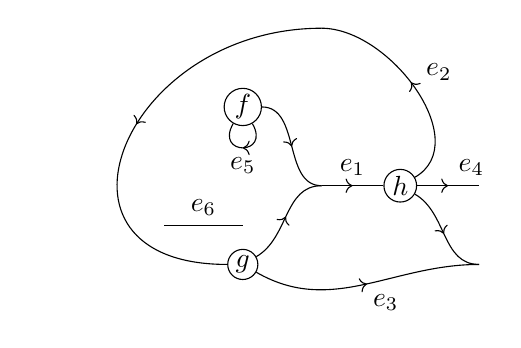
\begin{tikzpicture}
  \node[vertex] (f) at (0,1) {$f$};
  \node[vertex] (g) at (0,-1) {$g$};
  \node[vertex] (h) at (2,0) {$h$};
  \coordinate (e) at (1,0);
  \draw[edge] (f) to[out=0,in=180] (e);
  \draw[edge] (g) to[out=30,in=180] (e);
  \draw[edge] (e) to[out=0,in=180] node[auto] {$e_1$} (h);
  \coordinate (e2) at (1,2);
  \draw[edge] (h) to[out=30,in=0] node[auto,swap] {$e_2$} (e2);
  \draw[edge] (e2) to[out=180,in=180,looseness=2] (g);
  \coordinate (e3) at (3,-1);
  \draw[edge] (h) to[out=-30,in=180] (e3);
  \draw[edge] (g) to[out=-30,in=180] node[auto,swap] {$e_3$} (e3);
  \draw[edge] (h) -- node[auto,very near end] {$e_4$} +(1,0);
  \draw[edge] (f) to[out=-60,in=-120,looseness=5] node[auto] {$e_5$} (f);
  \draw (-1,-.5) -- node[auto] {$e_6$} (0,-.5);
\end{tikzpicture}
\]
Here $e_1$ is incident to $f$ and $g$ outgoing and to $h$ incoming, $e_2$ is incident to $h$ outgoing and $g$ incoming, $e_3$ is incident to $g$ and $h$ both outgoing, $e_4$ is incident to only $h$ outgoing, $e_5$ is incident to $f$ once outgoing and once incoming, and $e_6$ is not incident to any vertices at all.

There are many possible variations on hypergraphs.
Unlike in the combinatorial literature, but like the ``graphs'' usually used in category theory, our edges are not uniquely determined by the vertices they are incident to, i.e.\ we can have ``parallel edges''.
Also, we will assume that each vertex is incident to a finite set of edges, but in general place no such restriction on the edges; this will be convenient because it makes polygraphs a special case of directed hypergraphs.

We will also allow edges to contain ``loops''.
In particular, this distinguishes between the following two edges, neither of which is incident to any vertices, but of which one contains a loop and one does not:
\[
\begin{tikzpicture}
  \draw (0,0) -- (1,0);
  \draw (3,0) to[out=90,in=90,looseness=2] (4,0) to[out=-90,in=-90,looseness=2] (3,0);
\end{tikzpicture}
\]
Moreover, the hyper-ness of our graphs means that once we allow loops, we need to allow edges incident to vertices to also contain loops, and some edges to contain multiple loops.
The presence of loops turns out to make the definition of hypergraph very tricky to get right, in particular as regards the notion of morphism between such graphs.

First I tried just marking each edge with a natural number ``genus''; but in defining labeled hypergraphs as morphisms we need to be able to collapse loops, and automorphisms of hypergraphs need to be able to permute loops.
Then I thought of just assigning to each edge a pointed set of ``loops'', but when inserting one hypergraph into another we can create ``loops'' of a sort for which there is no obvious way to choose a ``basepoint'' to get an actual ``set of loops''; what arises naturally is a directed graph, or equivalently a free groupoid.
So I tried defining a hypergraph to have a (free) groupoid of edges rather than a set; but free groupoids have too many automorphisms.
At present the most promising approach seems to be to define a hypergraph to have a reflexive directed graph of edges, although the treatment of isomorphisms is perhaps still not completely satisfactory.

\begin{defn}
  A \textbf{hypergraph} $\G$ is a span
  \[ V \ot F \to E \]
  in which $V$ and $F$ are sets, each fiber of the map $F\to V$ is finite, and $E$ is a reflexive directed graph (with $F$ mapping into its vertices).

  The vertices of $E$ are called \textbf{edge representatives} of $\G$, the edges of $E$ are called \textbf{edge identifications} of $\G$, and the connected components of $E$ are called the \textbf{edges} of $\G$.
  The elements of $V$ are called the \textbf{vertices} of $\G$, and those of $F$ are called its \textbf{flags}.
  If a vertex and an edge (representative) are the image of a common flag, we say they are \textbf{incident}; thus the flags are the ``witnesses of incidence''.
  We also speak of a flag as being \textbf{incident} to its associated edge (representative) and vertex.
\end{defn}

We allow vertices that are not incident to any edges, and edges that are not incident to any vertices.
Also a vertex and an edge can be ``incident more than once'', i.e.\ the image of more than one common flag.

We write $\pi E$ for the set of edges, i.e.\ the set of connected components of $E$.

\begin{defn}
  Let $\G=(V\ot F\to E)$ be a hypergraph.
  \begin{itemize}
  \item The \textbf{degree} of a vertex in $\G$ is the cardinality of the set of flags incident to it, which is a natural number.
    The \textbf{rank} of an edge in $\G$ is the cardinality of the set of flags incident to it, which in general can be finite or infinite.
    We say $\G$ %has \textbf{finite rank} if all its ranks are finite, and $\G$
    is \textbf{finite} if $V$ and $E$ (hence also $F$) are finite.
  \item The free rank of the fundamental group of an edge (meaning that of its geometric realization, considered as a 1-truncated simplicial set, or equivalently of the free groupoid that it generates) is called its \textbf{genus}.
    We say $\G$ has \textbf{genus zero} if all of its edges have genus zero, i.e.\ $E$ is a forest.
  \item The \textbf{connected components} of $\G$ are the elements of the pushout of the span $V \leftarrow F \to \pi E$.
    We say $\G$ is \textbf{connected} if it has exactly one connected component.
    % In particular, vertices not incident to any edges, and edges not incident to any vertices, lie in their own connected components.
  \item We say $\G$ is \textbf{simple} if no edge is incident to any vertex more than once, so that the span $V \ot F \to \pi E$ is a relation.
  \item We say $\G$ is \textbf{reduced} if every edge has exactly one representative.
  \end{itemize}
\end{defn}

The ``hypergraphs'' of~\cite{glpn:directed-hypergraphs} are our finite simple reduced hypergraphs of genus zero.

\begin{defn}
  A \textbf{morphism of hypergraphs} is a diagram
  \[
  \begin{tikzcd}
    V' \ar[d] & F' \ar[d] \ar[r] \ar[l] \dlpullback[dl] & E' \ar[d]\\
    V  & F \ar[r] \ar[l] & E
  \end{tikzcd}
  \]
  in which $V'\to V$ and $F'\to F$ are functions, $E'\to E$ is a map of reflexive directed graphs, and the left-hand square is a pullback.
  This defines the category $\hy$.
\end{defn}

The fact that the left-hand square is a pullback means in particular that a morphism of hypergraphs preserves the degree of vertices.
However, it does not preserve the rank or the genus of edges.

Usually we will want to assume that the flags incident to each vertex are ordered so that we can distinguish them.
To say this precisely, let $\thy$ be the hypergraph with exactly one edge representative of genus zero, and for each natural number $n$ exactly one vertex incident to $n$ flags (each in turn incident to the unique edge representative).
We fix a labeling of these $n$ flags $0,1,\dots,n-1$, so that they are ordered.

\begin{defn}
  The category of \textbf{ordered hypergraphs} is the slice category $\hy/\thy$.
\end{defn}

A hypergraph morphism $\G\to\thy$ is uniquely determined on edges and vertices, so it consists only of the data of an ordering on the flags incident to each vertex.
Of course, such a morphism always exists, i.e.\ any hypergraph can be ordered; the point is that morphisms in $\hy/\thy$ must preserve the specified orderings.

\begin{comment}
Ordered hypergraphs have another convenient description.
Let $\Np$ be the set $\setof{(k,n) \in \N\times \N | k<n}$, with $\ell:\Np\to \N$ the second projection.
Thus the fiber of $\ell$ over $n\in\N$ is the canonical $n$-element linear order, and we can write $\thy = (\N \ot \Np \to 1)$.

Let $P_\ell$ be the polynomial endofunctor of $\Set$ defined by $\ell$, i.e.\ the composite
\[ \Set \xto{(\Np)^*} \Set/\Np \xto{\Pi_\ell} \Set/\N \xto{\Sigma_\N} \Set.\]
Thus an element of $P_\ell(E)$ is a finite list of elements of $E$.

Let $\RGph$ denote the category of reflexive directed graphs, with $U:\RGph\to\Set$ the functor taking the underlying set of vertices.

\begin{lem}
  The category $\hy/\thy$ of ordered hypergraphs is equivalent to the comma category
  \[
  \begin{tikzcd}
    \hy \ar[rr] \ar[d] \twocell{drr} && \Set \ar[d,equals] \\
    \RGph \ar[r,"U"'] & \Set \ar[r,"P_\ell"'] & \Set.
  \end{tikzcd}
  \]
\end{lem}
\begin{proof}
  An object of the comma category consists of a reflexive graph $E$ together with a set $V$ and a map $V \to P_\ell U E$.
  By definition of $P_\ell$, the latter map is equivalent to a map $f:V\to \N$ together with a map $f^*\Np \to UE$.
  This is exactly the data of a hypergraph $V \ot f^*\Np \to E$ equipped with a hypergraph map to $\thy = (\N \ot\Np \to 1)$.
\end{proof}

\begin{cor}
  $\hy/\thy$ is a presheaf topos.
  In particular, it is complete and cocomplete.
\end{cor}
\begin{proof}
  The functor $P_\ell \circ U : \RGph \to \Set$ is a parametric right adjoint, since $P_\ell$ is a polynomial functor and $U$ is a right adjoint.
  Thus, since $\RGph$ is a presheaf topos, by~\cite{cj:clfrag} $\hy/\thy$ is again a presheaf topos.
\end{proof}
\end{comment}

Sometimes we want a further refinement of ordered hypergraphs to \emph{directed} ones.
Let $\dhy$ denote the hypergraph with $E=1$ and $V=\N\times \N$, with the vertex $(n,m)$ having $n+m$ flags, which we think of as partitioned into $n$ ordered elements and $m$ ordered elements.

\begin{defn}
  The category of \textbf{directed hypergraphs} is the slice category $\hy/\dhy$.
\end{defn}

Thus, a directed hypergraph is a hypergraph in which at each vertex the list of incident flags is partitioned into two linear orders, which we call the \textbf{incoming} and \textbf{outgoing} flags respectively.
The numbers of incoming and outgoing flags are respectively called the \textbf{in-degree} and \textbf{out-degree} of the vertex.
Similarly, the \textbf{in-rank} and \textbf{out-rank} of an edge are respectively the cardinalities of the sets of outgoing (from their vertices, hence incoming to the edge) and incoming (to their vertices, hence outgoing from the edge) flags incident to it.

There is an obvious projection $\dhy\to\thy$ sending $(n,m)$ to $n+m$, with the incoming flags ordered before the outgoing ones.
Moreover, this has a section $\thy\to\dhy$ that sends the vertex $n$ to $(0,n)$.
Thus, we have
\[\hy/\dhy \simeq (\hy/\thy)/(\dhy\to\thy) \]
\[\hy/\thy \simeq (\hy/\dhy)/(\thy\to\dhy).\]
Thus, ordered and directed hypergraphs are each special cases of each other.

\begin{defn}
  A \textbf{cycligraph} is an ordered reduced hypergraph of genus zero.
  A directed cycligraph is called a \textbf{polygraph}.
  A polygraph in which each vertex has out-degree equal to 1 is a \textbf{multigraph}.

  In all of these cases, the edges are called \textbf{objects} and the vertices are called \textbf{morphisms}.
\end{defn}

A polygraph is the underlying data of a polycategory or a (colored) prop: each morphism has a finite list of ``source'' objects and a finite list of ``target'' objects.
Similarly, a multigraph is the underlying data of a multicategory: each morphism has a finite list of source objects and a single target object.
And a cycligraph is the underlying data of a cyclic multicategory, in which sources and targets are not distinguished; we speak instead of the \textbf{entries} of a morphism.

Our graph-theoretic representation of these objects invokes the Poincar\'e dual ``string diagram convention'', in which objects are 1-dimensional and morphisms are 0-dimensional.
The categories of cycligraphs, polygraphs, and multigraphs are presheaf toposes.
Also, cycligraphs are a reflective subcategory of $\hy/\thy$, and polygraphs are a reflective subcategory of $\hy/\dhy$.
We write $\pi \G$ for the cycligraph reflection of an ordered hypergraph $\G$, which has the same vertices and edges as $\G$ but its edge graph is the discrete set $\pi E$ of connected components of the edge graph $E$ of $\G$.

The above definitions of cycligraphs, polygraphs, and multigraphs make the following definitions very easy.

\begin{defn}\label{thm:labeled}
  If $P$ is a cycligraph, then a \textbf{$P$-labeled hypergraph} is a hypergraph $\G$ equipped with a hypergraph morphism $\G\to P$.
\end{defn}

Since a cycligraph is ordered, if $\G\to P$ is a $P$-labeled hypergraph then $\G$ automatically inherits an ordering.
On the other hand, if $\G$ is given as an ordered hypergraph, then to give a map $\G\to P$ is equivalently to give a map of cycligraphs $\pi \G \to P$.
Similar remarks apply to directed hypergraphs and polygraphs.

\begin{defn}
  A hypergraph $\G$ is \textbf{rooted} if it is equipped with a specified vertex $\ast_\G$ called the \textbf{root}.
  A morphism $\G\to\H$ of rooted hypergraphs is \textbf{strongly rooted} if the preimage of $\ast_\H$ is $\{\ast_\G\}$, i.e.\ the root and only the root is mapped to the root.
\end{defn}

In general, we think of the root as ``not really there'' and the flags incident to it as ``free''.
In a directed rooted hypergraph, we think of the incoming or outgoing edges of the root as ``incoming/outgoing to the entire graph''.
For instance, given the graph on the left with $\ast$ the root:
\begin{equation}
  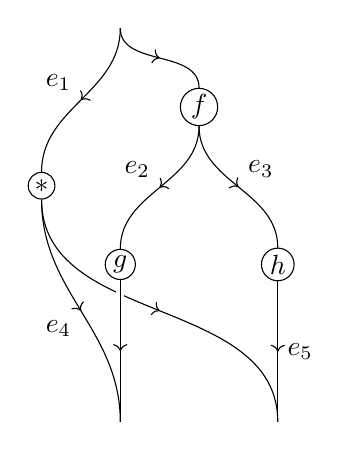
\begin{tikzpicture}
    \node[vertex] (r) at (0,0) {$\ast$};
    \node[vertex] (f) at (2,1) {$f$};
    \node[vertex] (g) at (1,-1) {$g$};
    \node[vertex] (h) at (3,-1) {$h$};
    \draw[edge] (1,2) to[out=-90,in=90] (f);
    \draw[edge] (1,2) to[out=-90,in=90] node[auto,swap] {$e_1$} (r);
    \draw[edge] (r) to[out=-90,in=90] (3,-3);
    \draw[edge] (h) to[out=-90,in=90] node[auto] {$e_5$} (3,-3);
    \draw[cross] (g) to[out=-90,in=90] (1,-3);
    \draw[edge] (g) to[out=-90,in=90] (1,-3);
    \draw[edge] (r) to[out=-90,in=90] node[auto,swap] {$e_4$} (1,-3);
    \draw[edge] (f) to[out=-90,in=90] node[auto,swap] {$e_2$} (g);
    \draw[edge] (f) to[out=-90,in=90] node[auto] {$e_3$} (h);
  \end{tikzpicture}
  \qquad
  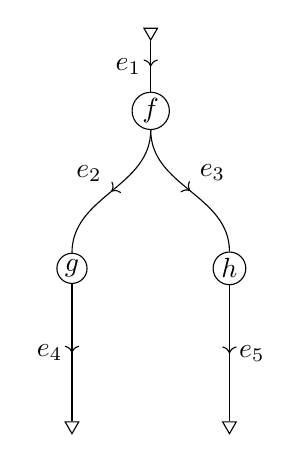
\begin{tikzpicture}
    \node[outer] (e1) at (2,2) {};
    \node[vertex] (f) at (2,1) {$f$};
    \node[vertex] (g) at (1,-1) {$g$};
    \node[vertex] (h) at (3,-1) {$h$};
    \node[outer] (e4) at (1,-3) {};
    \node[outer] (e5) at (3,-3) {};
    \draw[edge] (e1) to[out=-90,in=90] node[auto,swap] {$e_1$} (f);
    \draw[edge] (h) to[out=-90,in=90] node[auto] {$e_5$} (e5);
    \draw[edge] (g) to[out=-90,in=90] node[auto,swap] {$e_4$} (e4);
    \draw[edge] (f) to[out=-90,in=90] node[auto,swap] {$e_2$} (g);
    \draw[edge] (f) to[out=-90,in=90] node[auto] {$e_3$} (h);
  \end{tikzpicture}\label{eq:rooted-graph}
\end{equation}
we think of the edge $e_1$ as ``incoming to the graph'' and the edges $e_4,e_5$ as ``outgoing from the graph'', as drawn above on the right.

Note that an edge like $e_1$ that is ``incoming to the graph'' is \emph{incoming} to the root (as well as to other vertices like $f$), and one like $e_4$ or $e_5$ that is ``outgoing from the graph'' is \emph{outgoing} from the root (as well as from other vertices such as $g$ or $h$).
This choice, which as we will see makes the definition of insertion somewhat simpler, is only possible when using \emph{hyper}graphs, where edges can be incoming to multiple vertices and outgoing from multiple vertices.

% \begin{defn}\label{defn:loop}
%   A \textbf{loop} in a directed hypergraph is a sequence of flags
%   \[(f_0,g_0,f_1,g_1,\dots,f_n,g_n),\]
%   for $n\ge 0$, such that
%   \begin{enumerate}
%   \item Each $f_i,g_i$ are incident on the same edge, and
%   \item Each $g_i,f_{i+1}$ (including $g_n,f_0$ by mod-$n$ arithmetic) are incident on the same vertex, with $g_i$ incoming and $f_{i+1}$ outgoing.
%   \end{enumerate}
%   In particular, a loop with $n=0$ is an edge that is both incoming and outgoing to the same vertex.
%   A directed hypergraph is \textbf{loop-free} if it contains no loops.
% \end{defn}

% The left-hand rooted graph in~\eqref{eq:rooted-graph} is loop-free, which makes sense when considering the right-hand ``graph with free flags'' that it represents.
% If we chose to represent edges ``incoming to the graph'' by edges \emph{outgoing} to the root, then we would have to represent the right-hand ``graph with free flags'' in~\eqref{eq:rooted-graph} by the following rooted graph:
% \begin{equation}
%     \begin{tikzpicture}
%     \node[vertex] (r) at (0,0) {$\ast$};
%     \node[vertex] (f) at (2,1) {$f$};
%     \node[vertex] (g) at (1,-1) {$g$};
%     \node[vertex] (h) at (3,-1) {$h$};
%     \draw[edge] (r) to[out=90,in=90] node[auto] {$e_1$} (f);
%     \draw[edge] (h) to[out=-90,in=-90,looseness=2] node[auto] {$e_5$} (r);
%     \draw[edge] (g) to[out=-90,in=-90] node[auto,very near start] {$e_4$} (r);
%     \draw[edge] (f) to[out=-90,in=90] node[auto,swap] {$e_2$} (g);
%     \draw[edge] (f) to[out=-90,in=90] node[auto] {$e_3$} (h);
%   \end{tikzpicture}\label{eq:loop}
% \end{equation}
% which is not loop-free according to \cref{defn:loop} as written; thus we would have had to special-case the root vertex in \cref{defn:loop}.
% In fact, we regard~\eqref{eq:loop} as representing the following ``graph with free flags'':
% \begin{equation}
%   \begin{tikzpicture}
%     \node[vertex] (f) at (2,1) {$f$};
%     \node[vertex] (g) at (1,-1) {$g$};
%     \node[vertex] (h) at (3,-1) {$h$};
%     \draw[edge] (1,2) to[out=-90,in=90] (f);
%     \draw[edge] (1,2) to[out=-90,in=90] node[auto,swap,near end] {$e_1$} (-1,-4);
%     \draw[edge] (5,3) to[out=-90,in=90] node[auto] {$e_5$} (3,-3);
%     \draw[edge] (h) to[out=-90,in=90] (3,-3);
%     \draw[edge] (g) to[out=-90,in=90] (1,-3);
%     \draw[cross] (-1,3) to[out=-90,in=90] (1,-3);
%     \draw[edge] (-1,3) to[out=-90,in=90] node[auto,swap,near start] {$e_4$} (1,-3);
%     \draw[edge] (f) to[out=-90,in=90] node[auto,swap] {$e_2$} (g);
%     \draw[edge] (f) to[out=-90,in=90] node[auto] {$e_3$} (h);
%   \end{tikzpicture}\label{eq:loops2}
% \end{equation}
% in which $e_4$ and $e_5$ are ``incoming to the graph'' and $e_1$ is ``outgoing from the graph''.
% We do want to consider~\eqref{eq:loops2} as containing ``loops'', because there are paths from ``in'' to ``out'' that travel some paths ``backwards''.\fxnote{Is that right?}

Note also that we allow edges that are not incident to any vertices, or that are incident to only one vertex, but are \emph{not} incident to the root and hence not ``incoming'' or ``outgoing'' to the graph.
The following example shows a number of distinct degenerate possibilities in a directed (reduced) hypergraph (where $\ast$ is the root):
\begin{center}
  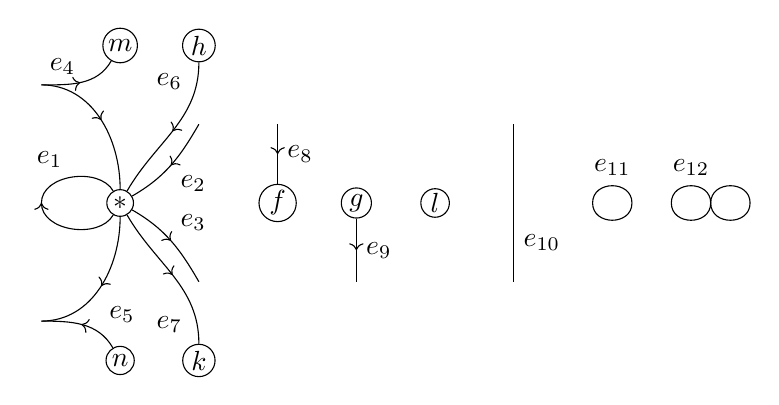
\begin{tikzpicture}
    \node[vertex] (r) at (0,0) {$\ast$};
    \draw[edge] (r) to[out=-120,in=-90] +(-1,0) to[out=90,in=120] node[auto] {$e_1$} (r);
    \draw[edge] (1,1) to[out=-120,in=30] node[auto] {$e_2$} (r);
    \draw[edge] (r) to[out=-30,in=120] node[auto] {$e_3$} (1,-1);
    \node[vertex] (h) at (1,2) {$h$};
    \draw[edge] (h) to[out=-90,in=60] node[auto,swap,near start] {$e_6$} (r);
    \node[vertex] (k) at (1,-2) {$k$};
    \draw[edge] (r) to[out=-60,in=90] node[auto,swap,near end] {$e_7$} (k);
    \node[vertex] (m) at (0,2) {$m$};
    \draw[edge] (-1,1.5) to[out=0,in=-120] node[auto,near start] {$e_4$} (m);
    \draw[edge] (-1,1.5) to[out=0,in=90] (r);
    \node[vertex] (n) at (0,-2) {$n$};
    \draw[edge] (n) to[out=120,in=0] node[auto,swap,near start] {$e_5$} (-1,-1.5);
    \draw[edge] (r) to[out=-90,in=0] (-1,-1.5);
    \node[vertex] (f) at (2,0) {$f$};
    \draw[edge] (2,1) -- node[auto] {$e_8$} (f);
    \node[vertex] (g) at (3,0) {$g$};
    \draw[edge] (g) -- node[auto] {$e_9$} +(0,-1);
    \node[vertex] (l) at (4,0) {$l$};
    \draw (5,1) -- node[auto,near end] {$e_{10}$} (5,-1);
    \draw (6.5,0) to[out=90,in=90,looseness=1.5] node[auto,swap] {$e_{11}$} (6,0) to[out=-90,in=-90,looseness=1.5] (6.5,0);
    \draw (7.5,0) to[out=90,in=90,looseness=1.5] node[auto,swap] {$e_{12}$} (7,0) to[out=-90,in=-90,looseness=1.5] (7.5,0);
    \draw (7.5,0) to[out=90,in=90,looseness=1.5] (8,0) to[out=-90,in=-90,looseness=1.5] (7.5,0);
  \end{tikzpicture}
\end{center}
Here $e_{10}$, $e_{11}$, and $e_{12}$ are all edges not incident to any vertices, with genera 0, 1, and 2 respectively.
We did not draw any arrows on them because only flags, not edges, are directed as ``incoming'' or ``outgoing''.
When interpreted as incoming or outgoing to the entire graph, the edges $e_1$--$e_7$ incident to the root above would be drawn as follows. %(preserving the ordering on incoming and outgoing edges to the root by drawing the incoming and outgoing edges to the graph in the same order).
\begin{center}
  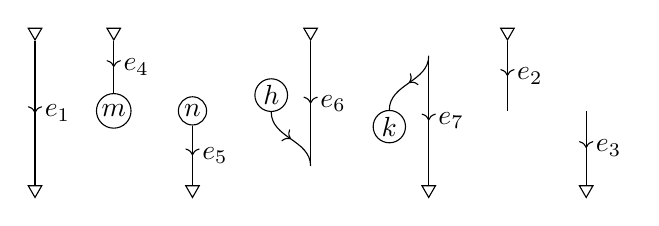
\begin{tikzpicture}
    \node[outer] (e1a) at (2,1) {};
    \node[outer] (e1b) at (2,-1) {};
    \draw[edge] (e1a) -- node[auto] {$e_1$} (e1b);
    \node[outer] (e2) at (8,1) {};
    \draw[edge] (e2) -- node[auto] {$e_2$} (8,0);
    \node[outer] (e3) at (9,-1) {};
    \draw[edge] (9,0) -- node[auto] {$e_3$} (e3);
    \node[vertex] (m) at (3,0) {$m$};
    \node[outer] (e4) at (3,1) {};
    \draw[edge] (e4) -- node[auto] {$e_4$} (m);
    \node[vertex] (n) at (4,0) {$n$};
    \node[outer] (e5) at (4,-1) {};
    \draw[edge] (n) -- node[auto] {$e_5$} (e5);
    \node[vertex] (h) at (5,.2) {$h$};
    \node[outer] (e6) at (5.5,1) {};
    \draw[edge] (e6) -- node[auto] {$e_6$} (5.5,-.7);
    \draw[edge] (h) to[out=-90,in=90]  (5.5,-.7);
    \node[vertex] (k) at (6.5,-.2) {$k$};
    \node[outer] (e7) at (7,-1) {};
    \draw[edge] (7,.7) -- node[auto] {$e_7$} (e7);
    \draw[edge] (7,.7) to[out=-90,in=90] (k);
  \end{tikzpicture}
\end{center}

We note that there are many ways in which an hypergraph (even an ordered one) can have nontrivial automorphisms.
One simple example is the graph with two vertices and no edges:
\begin{center}
\begin{tikzpicture}
  \node[circle,fill,inner sep=1pt] at (0,0) {};
  \node[circle,fill,inner sep=1pt] at (1,0) {};
\end{tikzpicture}
\end{center}
in which the two vertices can be swapped by an automorphism.
However, it is not necessary to be disconnected to have nontrivial automorphisms:
\begin{center}
  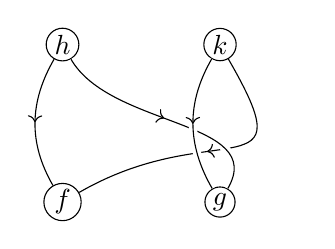
\begin{tikzpicture}[scale=2]
    \node[vertex] (f) at (0,0) {$f$};
    \node[vertex] (g) at (1,0) {$g$};
    \node[vertex] (h) at (0,1) {$h$};
    \node[vertex] (k) at (1,1) {$k$};
    \draw[edge] (h) to[out=-120,in=120] (f);
    \draw[edge] (k) to[out=-60,in=30,looseness=2] (f);
    \draw[cross] (h) to[out=-60,in=60] (g);
    \draw[edge] (h) to[out=-60,in=60] (g);
    \draw[cross] (k) to[out=-120,in=120] (g);
    \draw[edge] (k) to[out=-120,in=120] (g);
  \end{tikzpicture}
\end{center}
Here there is an automorphism that swaps $f$ with $g$ and swaps $h$ with $k$.
Moreover, if we orient this graph by giving the edges the left-to-right ordering in the picture, then this automorphism preserves the orientation.
This example cannot be rooted (the automorphism has no fixed points) --- or more precisely, it cannot occur in the connected component of the root --- but if we use edges that are incident on more than two vertices then we can have nontrivial automorphisms with fixed points:
\begin{center}
  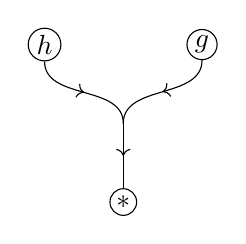
\begin{tikzpicture}
    \node[vertex] (f) at (0,0) {$\ast$};
    \node[vertex] (g) at (1,2) {$g$};
    \node[vertex] (h) at (-1,2) {$h$};
    \draw[edge] (g) to[out=-90,in=90] (0,1);
    \draw[edge] (h) to[out=-90,in=90] (0,1);
    \draw[edge] (0,1) -- (f);
  \end{tikzpicture}
\end{center}
Here there is an automorphism that swaps $g$ and $h$ and fixes the root $\ast$.
Note that this hypergraph is distinct from
\begin{center}
  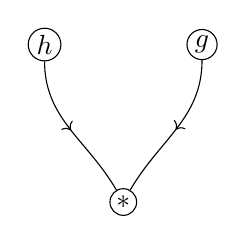
\begin{tikzpicture}
    \node[vertex] (f) at (0,0) {$\ast$};
    \node[vertex] (g) at (1,2) {$g$};
    \node[vertex] (h) at (-1,2) {$h$};
    \draw[edge] (g) to[out=-90,in=60] (f);
    \draw[edge] (h) to[out=-90,in=120] (f);
  \end{tikzpicture}
\end{center}
The former has \emph{one} edge that is incident to three vertices, while the latter has \emph{two} edges each incident to two vertices.
In contrast to the former, the latter has no automorphisms that preserve an ordering on the edges incident to the root.

The most restrictive thing we can say about about automorphisms is the following.

\begin{defn}
  A hypergraph is \textbf{binary}, or simply a \textbf{graph}, if % for each edge $e$ we have
  % \[ \rank(e) + 2 \cdot \genus(e)  = 2, \]
  % i.e.\ if
  every edge either has rank 2 and genus 0, or rank 0 and genus 1.
\end{defn}

Amusingly, this condition can be reformulated by saying that the rank of an edge is the same as its ``Euler characteristic'' $\chi=2-2g$.

\begin{lem}
  A connected rooted directed reduced binary hypergraph of genus zero has no nontrivial automorphisms.
\end{lem}
\begin{proof}
  Suppose $\phi$ is an automorphism of $\G$.
  By assumption, it must preserve the root.
  Since it is locally-ordered, it must preserve all edges incident to the root.
  But since each of those edges is incident to exactly one other vertex, it must preserve those vertices too.
  Proceeding inductively we find that it must preserve all edges and vertices in the connected component of the root, which is all of them since the graph is connected.
  Finally, since $\G$ is reduced and of genus zero, preserving all the edges means that it is the identity on the reflexive graph $E$.
\end{proof}

The presence of nontrivial automorphisms means that in general, we cannot simply ``pass to isomorphism classes'' of hypergraphs, and thus structures over hypergraphs are not definable using ``set-based shapes'', such as polynomial monads on the category of polygraphs.
In~\cite{bb:htapm} isomorphism classes and polynomial monads are shown to work for certain subclasses of graphs, but even when it works such a restriction is technical and error-prone.
Thus, we will generally work with categories instead of sets, never passing to isomorphism classes, and using a weak monad rather than a strict one.

In addition, our definition of hypergraph does not support all the isoomorphisms we would like to have.
For instance, we would like a non-reduced hypergraph to be isomorphic to a ``reduction'' in which distinct edge representatives of the same edge have been collapsed along an identification.
This collapse exists as a \emph{morphism} of hypergraphs in one direction, but is not invertible.
Thus we introduce the following definition:

\begin{defn}\label{defn:weq}
  A morphism of reflexive graphs is a \textbf{weak equivalence} if the preimage of every non-reflexivity edge is a singleton, and the preimage of every reflexivity edge is a nonempty undirected tree (equivalently, if its geometric realization is a homotopy equivalence).
  A morphism of hypergraphs is a \textbf{weak equivalence} if it is bijective on vertices (hence on flags) and its map on edges is a weak equivalence.
\end{defn}

\begin{lem}\label{thm:reduction}
  Every hypergraph admits a weak equivalence to a reduced one.
  Moreover, if $\G\to \G_1$ and $\G \to \G_2$ are weak equivalences with $\G_1$ and $\G_2$ reduced, then there is a non-unique isomorphism $\G_1 \cong \G_2$ (which need not commute with the maps from $\G$).
\end{lem}
\begin{proof}
  To construct a reduction of $\G$, choose a spanning tree inside each edge and collapse it to a point.
  The second statement follows since weak equivalences induce isomorphisms of sets of edges that preserve genera, and any two reduced hypergraphs with the same vertices, flags, edges, and genera are isomorphic.
\end{proof}

The non-uniqueness of ``reduction'' is the reason for including non-reduced graphs in the theory; as we will see, they arise naturally in the construction of insertion in \cref{sec:tt-insertion}, and without a canonical way to reduce them it is more natural to keep them around.
If we represented the edges by a free groupoid rather than a reflexive graph, weak equivalences would be actual equivalences, but free groupoids also have additional automorphisms that we don't want.

% The directed version of the binary condition is a little kludgy to state due to our convention about the orientations of flags incident to the root.

% \begin{defn}
%   Let $\G$ be a directed rooted hypergraph.
%   \begin{enumerate}
%   \item $\G$ is \textbf{weakly binary} if it is binary (in the undirected sense) and moreover every edge not incident to the root has equal in-rank and out-rank (i.e.\ either both 1 or both 0).
%   \item $\G$ is \textbf{strongly binary} if it is binary (in the undirected sense) and moreover if we switched the direction of all flags incident to the root then every edge would have equal in-rank and out-rank.
%   \end{enumerate}
% \end{defn}

% Here is an example of a strongly binary directed rooted hypergraph:
% \[
% \begin{tikzpicture}
%   \node[vertex] (f) at (0,0) {$f$};
%   \node[vertex] (g) at (1,-1) {$g$};
%   \node[vertex] (h) at (0,-2) {$h$};
%   \node[outer] (in1) at (0,1) {};
%   \node[outer] (in2) at (2,1) {};
%   \node[outer] (in3) at (1,1) {};
%   \node[outer] (out2) at (2,-3) {};
%   \node[outer] (out3) at (1,-3) {};
%   \node[outer] (out1) at (0,-3) {};
%   \draw[edge] (f) -- (g);
%   \draw[edge] (in1) -- (f);
%   \draw[edge] (g) -- (h);
%   \draw[edge] (f) -- (h);
%   \draw[edge] (h) -- (out1);
%   \draw[edge] (in3) -- (g);
%   \draw[edge] (in2) -- (out2);
%   \draw[edge] (h) -- (out3);
% \end{tikzpicture}
% \]
% Here is one that is weakly binary but not strongly binary:
% \[
% \begin{tikzpicture}
%   \node[vertex] (f) at (0,0) {$f$};
%   \node[vertex] (g) at (1,-1) {$g$};
%   \node[vertex] (h) at (0,-2) {$h$};
%   \node[outer] (in1) at (0,1) {};
%   \node[outer] (in2) at (3,1) {};
%   \node[outer] (in4) at (2,1) {};
%   \node[outer] (in3) at (1,1) {};
%   \node[outer] (out2) at (3,-4) {};
%   \node[outer] (out3) at (1,-4) {};
%   \node[outer] (out4) at (2,-4) {};
%   \node[outer] (out1) at (0,-4) {};
%   \draw[edge] (f) -- (g);
%   \draw[edge] (in1) -- (f);
%   \draw[edge] (g) -- (h);
%   \draw[edge] (f) -- (h);
%   \draw[edge] (h) -- (out1);
%   \draw[edge] (in3) -- (g);
%   \draw[edge] (in2) -- (out2);
%   \coordinate (four) at (1,-3);
%   \draw[edge] (h) to[out=-90,in=90] (four);
%   \draw[edge] (in4) to[out=-90,in=90] (four);
%   \coordinate (five) at (2,-3);
%   \draw[edge] (five) to[out=-90,in=90] (out3);
%   \draw[edge] (five) to[out=-90,in=90] (out4);
% \end{tikzpicture}
% \]
% And here is a directed rooted hypergrah that is binary in the undirected sense, but not even weakly binary in the directed sense:
% \[
% \begin{tikzpicture}
%   \node[vertex] (f) at (0,0) {$f$};
%   \node[vertex] (g) at (1,-1) {$g$};
%   \node[vertex] (h) at (0,-2) {$h$};
%   \node[outer] (in1) at (0,1) {};
%   \node[outer] (in3) at (1,1) {};
%   \node[outer] (out3) at (1,-4) {};
%   \node[outer] (out1) at (0,-4) {};
%   \draw[edge] (f) -- (g);
%   \draw[edge] (in1) -- (f);
%   \draw[edge] (g) -- (h);
%   \draw[edge] (h) -- (out1);
%   \draw[edge] (in3) -- (g);
%   \draw[edge] (h) -- (out3);
%   \coordinate (two) at (-1,-3);
%   \draw[edge] (f) to[out=-90,in=90] (two);
%   \draw[edge] (h) to[out=-120,in=90] (two);
% \end{tikzpicture}
% \]

We end this section by comparing our graphs to others in the literature.
Graphs with ``free flags'' have been used in defining many kinds of operads, but usually only of the binary sort, corresponding to non-cartesian multicategories and operads.

In a reduced binary rooted hypergraph, we can define an involution on the set of flags not incident to the root by sending each flag to the other flag of its corresponding edge, if that flag is not incident to the root, or to itself otherwise.
The quotient of this involution is then isomorphic to the set of edges that are incident to some non-root vertex.
Thus, we can equivalently define a binary rooted hypergraph by giving
\begin{itemize}
\item a set $F$ of flags (the flags not incident to the root),
\item an involution on $F$,
\item a set of ``exceptional linear edges'' (the edges incident to the root twice),
\item a set of ``exceptional loops'' (the edges not incident to any vertex --- the only ones with genus 1), and
\item a set $V$ of (non-root) vertices and a function $F\to V$ with finite linearly ordered fibers (equivalently, a ``partition'' of $F$ into finite linearly ordered blocks, some of which are allowed to be empty).
\end{itemize}
This is the definition of ``graph'' used commonly in operad theory, e.g.~\cite{bm:gen-opds,km:gwcqceg,costello:ainf,mms:wheeled-props,gk:modular-operads}, although often exceptional loops and edges are omitted or treated inconsistently.

Alternatively, if we remove the root but not the flags incident to it, then the function $F\to V$ becomes a partial function, which is defined on a flag just when that flag is not incident to the root.
Now we still have the exceptional edges (those incident to two flags that are not incident to any vertices) and the exceptional loops (those not incident to any flags).
This is essentially how binary rooted hypegraphs are encoded in~\cite{bb:htapm}, except that their exceptional loops are ``incident to a single flag twice'' rather than to no flags at all.

Another possibility is to express the partial function $F\rightharpoonup V$ as a relation, i.e.\ a span $F \ot H \to V$ in which $H\to F$ is injective.
If we exclude the possibility of exceptional loops, then the function $F\to E$ is a 2-to-1 surjection and hence can be encoded up to isomorphism by a fixed-point-free involution of $F$.
This is the definition of graph from~\cite{jk:feynman} (though they call the elements $H$ the ``flags'' and those of $F$ the ``(directed) edges'').
Their graph morphisms are similar to ours, although theirs are not required to preserve the ``degree of the root''.


\section{Type theory for hypergraphs}
\label{sec:tt-hy}

For all of this section, let $P$ be a fixed cycligraph; we will describe a type theory for $P$-labeled hypergraphs.
This includes unlabeled hypergraphs as the degenerate case when $P$ is terminal, and also the directed case if $P$ happens to be a polygraph or a multigraph.

An \textbf{edge context} $\Delta$ is a finite list of distinct variables, each labeled with an object of $P$ as its type.

\begin{mathpar}
  \inferrule{ }{\ec \edgectx}
  \and
  \inferrule{\Delta\edgectx \\ p\in P \\ x\notin \Delta}{(\Delta,x:p) \edgectx}
\end{mathpar}

A \textbf{loop context} $\Xi$ in an edge context $\Delta$ is a finite list of equalities between variables of the same type.

\begin{mathpar}
  \inferrule{ }{\Delta \types \ec\loopctx}
  \and
  \inferrule{\Delta\types\Xi\loopctx \\ (x:p)\in \Delta \\ (y:p)\in\Delta}{\Delta\types (\Xi,x\doteq y) \loopctx}
\end{mathpar}

A \textbf{vertex} in an edge context is a morphism of $P$ with variables of appropriate type assigned as its entries.

\begin{mathpar}
  \inferrule{\alpha\in P(p_1,\dots,p_n) \\ (x_i:p_i)\in\Delta}{\Delta \types \alpha(x_1,\dots,x_n) \vertex}
\end{mathpar}

In the directed case, we write $\alpha(x_1,\dots,x_n ; y_1,\dots,y_m)$ to indicate the separation of entries into domain and codomain.

A \textbf{graph context} is an edge context, a loop context, and a finite list of variables assigned to vertices.

\begin{mathpar}
  \inferrule{\Delta \edgectx \\ \Delta\types \Xi\loopctx}{\Delta \mid\Xi\types \ec\graph}
  \and
  \inferrule{\Delta \mid\Xi\types \Theta\graph \\ \Delta\types M\vertex \\ (f\notin \Theta)}{\Delta\mid\Xi\types (\Theta,f:M)\graph}
\end{mathpar}

\begin{thm}\label{thm:ctx-hy}
  A graph context determines, and is determined by, a finite $P$-labeled hypergraph $\G\to P$.
\end{thm}
\begin{proof}
  The variables in the edge context correspond to the edge representatives, and their assignment to types corresponds to the action of the labeling morphism $\G\to P$ on these.
  The equalities in the loop context correspond to non-reflexivity edges in the reflexive graph $E$.
  The variables in the graph context correspond to the vertices of $\G$, and their type assignment to a morphism of $P$ is the action of $\G\to P$ on vertices.
  Finally, the list of variables in a syntactic vertex $\alpha(x_1,\dots,x_n)$ specifies the flags of $\G$.
\end{proof}

In order to enhance \cref{thm:ctx-hy} to some sort of equivalence, we need to introduce morphisms between graph contexts.

\begin{defn}
  Given two graph contexts
  \begin{mathpar}
    \Delta\mid\Xi\types \Theta\graph \and
    \Delta'\mid\Xi'\types \Theta'\graph \and
  \end{mathpar}
  a \textbf{context morphism} or \textbf{substitution} $(\sigma\mid\tau\mid\nu):(\Delta\mid\Xi\mid\Theta)\to(\Delta'\mid\Xi'\mid\Theta')$ consists of:
  \begin{enumerate}
  \item A function $\sigma : \Delta' \to \Delta$ that respects types.
  \item A partial function $\tau : \Xi' \rightharpoonup \Xi$ such that
    \begin{enumerate}
    \item If $\tau(x\doteq y)$ is defined, then it is of the form $\sigma(x)\doteq \sigma(y)$.
    \item If $\tau(x\doteq y)$ is undefined, then $\sigma(x)=\sigma(y)$.
    \end{enumerate}
  \item A function $\nu : \Theta' \to \Theta$ that respects types modulo $\sigma$, i.e.\ if $f:\alpha(\vec x)$ then $\nu(f) : \alpha(\sigma(\vec x))$.
  \end{enumerate}
  This defines the category $\GCtx_P$ of $P$-labeled graph contexts.
\end{defn}

\begin{thm}\label{thm:hyctx}
  There is an equivalence of categories
  \[ (\hy/P)\op \simeq \GCtx_P. \]
\end{thm}
\begin{proof}
  The contravariance of the equivalence is because context morphisms were defined to go the opposite way from their underlying functions on contexts (we think of the morphism as substituting $\sigma(x)$ for $x$ and so on).
  The function $\sigma$ corresponds to the map on edge representatives and the function $\nu$ corresponds to the map on vertices.
  The partial function $\tau$ corresponds to the action on edge identifications; where it is undefined, we send the corresponding edge to reflexivity.
\end{proof}

We should also be able to define the context morphisms more type-theoretically as an inductive judgment, but I will not do that right now.
However, it is useful to characterize the weak equivalences from \cref{defn:weq} in such a way, and the result is quite natural: they are obtained by repeatedly substituting along equalities of \emph{distinct} variables.
\begin{equation}\label{eq:subst}
  \inferrule{\Delta,y:p\mid\Xi,x\doteq y \types \Theta\graph \\ x\not\jdeq y}{\Delta\mid\Xi[x/y]\types \Theta[x/y] \graph}
\end{equation}
An inductive characterization of these context morphisms, using a judgment
\begin{equation}
  (\sigma\mid\tau\mid\nu):(\Delta\mid\Xi\mid\Theta)\to(\Delta'\mid\Xi'\mid\Theta') \weq\label{eq:weq}
\end{equation}
is given by
\begin{mathpar}
  \inferrule{ }{(1_\Delta\mid 1_\Xi\mid 1_\Theta) : (\Delta\mid\Xi\mid\Theta)\to (\Delta\mid\Xi\mid\Theta)\weq}
  \and
  \inferrule{(\sigma\mid\tau\mid\nu) : (\Delta\mid\Xi\mid\Theta)\to (\Delta'\mid\Xi'\mid\Theta')\weq
  \\ x\not\jdeq y}
  {(\sigma,[y\mapsto x]\mid \tau\mid\nu) : (\Delta,y:p\mid\Xi,x\doteq y\mid\Theta)\to (\Delta'\mid\Xi'\mid\Theta')\weq}
  \and
  \inferrule{(\sigma\mid\tau\mid\nu) : (\Delta\mid\Xi\mid\Theta)\to (\Delta'\mid\Xi'\mid\Theta')\weq
  \\ x\not\jdeq y}
  {(\sigma,[x\mapsto y]\mid \tau\mid\nu) : (\Delta,x:p\mid\Xi,x\doteq y\mid\Theta)\to (\Delta'\mid\Xi'\mid\Theta')\weq}
\end{mathpar}


\section{Insertion of hypergraphs}
\label{sec:insertion}

We now define an operation of \emph{insertion} of hypergraphs, which replaces some of the vertices in one graph by entire new graphs having the same ``flag structure''.
To clarify the abstract properties of this operation, we phrase it as a bicategorical composition.

\begin{defn}
  If $E_1 \xot{s} F \xto{t} E_2$ is a span of reflexive graphs in which $F$ is discrete (has only reflexivity edges), then its \textbf{collage} $E_1 \coll_F E_2$ is the disjoint union reflexive graph $E_1+E_2$ augmented by a new edge for each $x\in F$, attaching $s(x)$ to $t(x)$.
\end{defn}

\begin{defn}
  A \textbf{corolla} is a reduced hypergraph of genus zero of the form $1 \ot F = F$, i.e.\ having one vertex, each flag of which is incident to a unique edge.
  A disjoint union of corollas, i.e.\ a hypergraph of the form $V \ot F = F$, is called an \textbf{inflorescence}.\footnote{A corolla is the whorl of petals in a flower; an inflorescence is a cluster of flowers on a single stem.}
\end{defn}

Note that an inflorescence is uniquely determined, up to non-unique isomorphism, by giving a set of vertices and their degrees.

\begin{defn}
  A \textbf{conormal lax bicategory} is like a bicategory, but its unit transformations $f \circ 1_x \to f$ and $1_y\circ f \to f$ are not necessarily invertible (though it associativity isomorphisms are).
  We still ask for the same coherence axioms.
\end{defn}

\begin{thm}\label{thm:hyrel}
  There is a conormal lax bicategory $\hyrel$ in which
  \begin{itemize}
  \item The objects are inflorescences.
  \item The morphisms from $\A$ to $\B$ are cospans $\A \to \G \ot \B$ of hypergraphs such that $(\A+\B) \to \G$ is bijective on vertices.
    Equivalently, the morphisms are hypergraphs $\G$ equipped with a partition of their vertices into two disjoint subsets; the inflorescences $\A$ and $\B$ are then uniquely determined.
  \item The composite $\G \coll_{\B} \H$ of $\A \to \G \ot \B$ and $\B \to \H \ot \C$ is defined to be
    \[ V_{\A}  + V_{\C} \longleftarrow F_{\A} + F_{\C} \longrightarrow E_{\G} \coll_{E_\B} E_{\H} \]
    In other words:
    \begin{enumerate}
    \item The vertices and flags of $\G \coll_{\B} \H$ are the disjoint unions of those of $\A$ and those of $\C$.
    \item The edge graph of $\G \coll_{\B} \H$ is the collage of those of $\G$ and $\H$ under that of $\B$.
      Thus, an edge representative is either one in $\G$ or one in $\H$, while an edge identification is either one in $\G$, one in $\H$, or one identifying the images in $\G$ and $\H$ of an edge in $\B$.
    \end{enumerate}
  \item The unit $1_{\A}$ of an inflorescence $\A=(V\ot F = F)$ is $V+V \ot F+F \to F$, with the two evident inclusions from $\A$.
  \end{itemize}
\end{thm}
\begin{proof}
  Associativity follows from the associativity of coproducts and collages.
  The latter means that if we have $E_1 \ot F_1 \to E_2 \ot F_2 \to E_3$ with $F_1,F_2$ discrete, then $(E_1 \coll_{F_1} E_2) \coll_{F_2} E_3 \cong E_1 \coll_{F_1} (E_2 \coll_{F_2} E_3)$, and the pentagon equation is satisfied if we have another span $E_3 \ot F_3 \to E_4$.
  This is a straightforward verification.

  The composite $1_{\A} \coll_{\A} \G$ has the same vertices and flags as $\G$ (up to isomorphism), but its edge graph has been augmented by a new edge representative $\bar{x}$ for each flag $x\in F_{\A}$, and new identifications connecting $\bar{x}$ to the edge representative incident to the image of $x$ in $\G$.
  Thus, it is not isomorphic to $\G$, but admits a map to $\G$ that contracts each of these new identifications to reflexivity.
  The other unit constraint is dual, and the coherence axiom is straightforward to check.
\end{proof}

Note that if $\A$ and $\C$ are ordered or directed, so is $\G \coll_{\B} \H$, since its vertices are simply those of $\A$ and $\C$.
Moreover, the set $\pi(E_1 \coll_F E_2)$ of connected components of a collage of reflexive graphs is the pushout $\pi E_1 +_{\pi F} \pi E_2$.
It follows that in the ordered case, the cycligraph reflection $\pi(\G \coll_{\B} \H)$ of a composite in $\hyrel$ is the pushout $\pi\G +_{\pi \B} \pi \H_v$ of the cycligraph reflections, and similarly for the unit.
In other words, the ``homwise cycligraph reflection'' of the ordered form of $\hyrel$ is simply the bicategory of cospans of cycligraphs.

The most common situation in which we apply this is the following.
Suppose $\G = (V\ot F \to E)$ is a hypergraph, and that for some subset $V_0 \subseteq V$ and each $v\in V_0$ we have a rooted hypergraph $\H_v = (V_v \ot F_v \to E_v)$ whose root $\ast_v$ has the same degree as $v$.
%In the directed case, we require it to have the same in-degree and out-degree separately.
(Usually, $V_0$ will be either a single vertex or the set of all non-root vertices.)

We regard $\G$ as a morphism from $\A$ to $\B$ in $\hyrel$, where $\A$ is determined by the vertices not in $V_0$ and $\B$ is determined by the vertices in $V_0$.
Similarly, we regard $\sum_v \H_v$ as a morphism from $\B'$ to $\C$, where $\B'$ is determined by the roots $\setof{ \ast_v | v\in V_0}$ and $\C$ by the non-root vertices.
The assumption tells us that $\B'\cong \B$, so we can form the composite $\G \coll_{\B} \sum_v \H_v$ in $\hyrel$.
We call the result the \textbf{insertion} of the hypergraphs $\H_v$ into $\G$ at the vertices $v\in V_0$, denoted $\ins{\G}{V_0}{v}{\H_v}$.

If $\G$ was rooted with $\ast \notin V_0$, then $\ins{\G}{V_0}{v}{\H_v}$ is again rooted with the same root.
Moreover, if $\G$ and each $\H_v$ are labeled by some cycligraph $P$, with labelings that agree on $V_0$, then since these labelings factor through $\pi \G$ and $\pi \H_v$ and the cycligraph reflection takes insertions to pushouts, there is a unique induced labeling on $\ins{\G}{V_0}{v}{\H_v}$.

\fxnote{Add some examples.}



\section{Type theory for insertion}
\label{sec:tt-insertion}

If $\Theta$ and $\Theta'$ are graph contexts, we write $\Theta \sametypes \Theta'$ to mean that their variables have the same types in the same order, i.e.:
\begin{mathpar}
  \inferrule{ }{\Delta\mid\Xi\types \ec \sametypes \ec}
  \and
  \inferrule{\Delta\mid\Xi\types \Theta\sametypes\Theta' \\ \Delta\types \alpha(\vec x)\vertex \\ \Delta\types \alpha(\vec y) \vertex}{\Delta\mid\Xi\types (\Theta,\alpha(\vec x)) \sametypes (\Theta',\alpha(\vec y))}
\end{mathpar}
We also write $\varsof\Theta$ for the ordered list of edge variables occurring in $\Theta$, i.e.:
\begin{align*}
  \varsof\ec &\coloneqq ()\\
  \varsof{(\Theta,\alpha(\vec x))} &\coloneqq (\varsof\Theta,\vec x)
\end{align*}
And if $\vec x=(x_1,\dots,x_n)$ and $\vec y=(y_1,\dots,y_n)$ are lists of variables of the same length (such as $\varsof\Theta$), then by $\vec x \doteq \vec y$ we mean the list of equalities
\[x_1\doteq y_1,\dots,x_n\doteq y_n.\]
With these notations, the insertion rule can be expressed as:
\begin{mathpar}
  \inferrule{\Delta\mid\Xi\types (\Theta,\Phi)\graph\\ \Delta'\mid\Xi'\types (\Psi,\Upsilon) \graph \\ \Phi\sametypes\Psi}
  {\Delta,\Delta' \mid \Xi,\Xi',\varsof\Phi\doteq\varsof\Psi \types (\Theta,\Upsilon) \graph}
\end{mathpar}
Implicit in the notation is that $\Delta\cap \Delta'=\emptyset$, so that $\varsof\Phi\doteq\varsof\Psi$ consists of equalities between distinct variables.
Thus at least some of them can be substituted away by a weak equivalence as in~\eqref{eq:subst} (a ``nondeterministic unification algorithm'' for the arguments of the vertices in $\Phi$ and $\Psi$).
However, we may still be left with additional self-loops created by the insertion, for instance:

\begin{mathpar}
  \inferrule*{\inferrule*{x:p \mid\cdot \types (\Theta_1,f:\alpha(x,x)) \graph \\
    u:p \mid\cdot \types (g:\alpha(u,u),\Theta_2) \graph}
  {x:p,u:p \mid x\doteq u, x\doteq u \types (\Theta_1,\Theta_2)\graph}}
{x:p \mid x\doteq x \types \Theta_1,\Theta_2[x/u] \graph}
\end{mathpar}


\section{Hypercategories and virtual hypercategories}
\label{sec:hypercats}

We now construct a monad $T$ (in fact, several monads) out of hypergraphs.
Rather than an ordinary monad on a 1-category (such as polygraphs or cycligraphs), our monad must be a 2-monad on a 2-category, since it will incorporate the automorphisms of hypergraphs so that $T P$ will not be discrete even if $P$ is.
In fact, $T P$ will also include the weak equivalences from \cref{defn:weq}, so that it will not even be a groupoid.

In all the semantic examples that we know, these weak equivalences act as isomorphisms; so in constructing the monad we could formally invert them.
But this would actually make our lives \emph{more} difficult, since it would be extra work to verify that the inversion is consistent everywhere, and from a syntactic point of view it is more natural to keep them directional (since substitution is more natural than its inverse).
Moreover, we will also define ``cartesian'' variants of $T$ that include morphisms of hypergraphs that are not even weak equivalences, so it is more consistent to keep everything noninvertible.
However, this choice does mean that $T$ will only be a lax monad, just as $\hyrel$ is only a lax bicategory.

\begin{anfxnote}{Technology}
  I am currently working on some technology (``parametric right 2-adjoints'') that should make it easier to construct these monads explicitly.
  For now let's not worry about the details.
\end{anfxnote}

Let $J$ be the category such that presheaves on $J$ are cycligraphs.
Then $J$ has one object $\bullet$ and objects $[n]$ for $n\in\N$, with $n$ nonidentity morphisms $\bullet\to [n]$.
A functor $J\op\to\Cat$ is an internal cycligraph in \Cat, or equivalently an internal category in cycligraphs; we call it a \textbf{\Cat-cycligraph}.
A \Cat-cycligraph has four kinds of data: the objects and arrows of the category $P(\bullet)$, which we call \emph{objects} and \emph{arrows} of $P$, and the objects and arrows of the categories $P([n])$, which we call \emph{morphisms} and \emph{2-cells} of $P$.
The $n$ objects associated to a morphism, and the $n$ arrows associated to a 2-cell, are called its \emph{entries}.

\begin{comment}
By an \textbf{$n$-hypergraph} we will mean a rooted ordered hypergraph whose root has rank $n$.
We define a \Cat-cycligraph $J\op\to\Cat$ by sending $[n]$ to the category of $n$-hypergraphs and weak equivalences between them, and $\bullet$ to the terminal category with unique object $\star$.
(Note that any isomorphism is a weak equivalence.)
Let $p:K_1 \to J$ be the (split, but not discrete) fibration corresponding to this functor; thus it is the category of rooted ordered hypergraphs and weak equivalences with an additional object $\star$ adjoined along with $n$ morphisms from $\ast$ to each $n$-hypergraph ``picking out the edges incident to the root''.

We define a profunctor $H_1 : J\op\times K_1 \to \Set$ as follows:
\begin{align*}
  H_1(\bullet,\G) &= \text{edges of $\G$}\\
  H_1([n],\G) &= \text{non-root vertices in $\G$ with rank $n$}\\
  H_1(\bullet,\star) &= 1\\
  H_1([n],\star) &= \emptyset
\end{align*}
The morphisms of graphs in the fibers of $K_1$ over $[n]$ act (by isomorphisms) on $\H_1(-,\G)$ in the obvious way.
The $n$ morphisms $\star\to\G$ in $K_1$ induce the maps $H_1(\bullet,\star) \to H_1(\bullet,\G)$ picking out the edges incident to the root.
The $n$ morphisms $\bullet\to [n]$ in $J$ induce the maps $H_1([n],\G) \to H_1(\bullet,\G)$ selecting the edges incident to each vertex.

Thus we have an induced p.r.a.\ endo-2-functor $T_1$ of the 2-category $[J\op,\Cat]$ of \Cat-cycligraphs.
If $P$ is a cycligraph, then the objects of $T_1 P$ are those of $P$, while a morphism in $T_1 P$ with arity $n$ consists of a rooted ordered $n$-hypergraph $\G$ (an object of $K_1$) and a natural transformation $H_1(-,\G) \to P$, which is to say a $P$-labeling of the non-root vertices in $\G$.
If $P$ is a $\Cat$-cycligraph, then this definition extends functorially to the category of objects and the category of morphisms.

We now make $T_1$ into a sort of monad, using \cref{thm:pra-psfr}.

The identity functor $\Id$ of $[J\op,\Cat]$ is p.r.a.\ and determined by the hom-profunctor $\hom_J$ and the identity split fibration $J\to J$.
Thus, to define a unit $\eta : \Id \to S$, it suffices to define a functor $k:J\to K_1$ such that $p k\cong 1_J$ and $H_1(1,k) \cong \hom_J$.
In our case, we define $k$ to send $\bullet$ to $1$ and $[n]$ to the \textbf{rooted $n$-corolla} $\C_n$, which has two vertices (one of which is the root) and $n$ edges each incident to both vertices once in the same order.
It is clear that $k$ is a section of $p$, while inspecting the definition of $H_1$ yields $H_1(1,k) \cong \hom_J$.

Thus we have a cartesian 2-natural transformation $\eta : \Id\to T_1$, where $\eta_P : P \to T_1 P$ sends each each morphism to the $n$-corolla labeled by itself.
Of course, there are many different (isomorphic) $n$-corollas.
However, onec we fix any particular such corolla for each $n$, we get such a transformation $\eta$.
The existence of other corollas means that $\eta$, though fully faithful, is not replete: objects of $T_1 P$ defined using other corollas are isomorphic to ones in the image of $\eta$ but are not in the image of $\eta$ themselves.

Next we define a cartesian 2-natural transformation $\mu:T_1 T_1\to T_1$.
As constructed in \cref{thm:pracomp2}, the composite $T_1 T_1$ is determined as follows: first we form $\hom_J(H_1,K_1)$, incarnate it as a split fibration $L_1 \to K_1$, and then take the composites $L_1\to K_1\to J$ and $H_1 \otimes_{K_1} M_1$ for the profunctor $M_1$ defined as there.

Now by definition, an object of $L_1$ is (either $\star$ or) a rooted ordered hypergraph $\G$ each of whose non-root vertices $v$ is labeled by another rooted ordered hypergraph $\H_v$, with an ordered bijection between the flags of $v$ and of $\ast_v$.
Thus we can form $\ins{\G}{V_0}{v}{\H_v}$, giving a functor $k:L_1 \to K_1$ over $J$.

Now we have to unravel the profunctor $M_1 : K_1\op \times L_1 \to \Cat$.
In the notation of \cref{thm:pracomp}, with $\ell = (\G,\{\H_v\})$, the objects of $F_\ell$ are the edges and non-root vertices of $\G$, with morphisms to each vertex from its incident edges.
The functor $\hat\ell : F_\ell \to K_1$ sends each vertex $v$ to the hypergraph $\H_v$, and each edge to $\star$.
Thus, an object of $G_\ell$ is either $\star$ together with an edge of $\G$, or a rooted ordered hypergraph $\G'$ with a weak 

 actually lands in $\Set$ and is defined as follows:
\begin{align*}
  M_1(\G',(\G,\H_v)) &= \text{weak equivalences $\G'\to \H_v$ for some $v$}\\
  M_1(\star,(\G,\H_v)) &= \text{edges of $\G$}\\
  M_1(\G',\star) &= \emptyset\\
  M_1(\star,\star) &= 1\\
\end{align*}
We claim that the composite profunctor $H_1 \otimes_{K_1} M_1$ is then given by
\begin{align*}
  H_1 \otimes_{K_1} M_1(\bullet,(\G,\H_v)) &= \text{edges of $\H_v$ for some $v$}\\
  H_1 \otimes_{K_1} M_1([n],(\G,\H_v)) &= \text{non-root vertices in $\H_v$ for some $v$ with rank $n$}\\
  H_1 \otimes_{K_1} M_1(\bullet,\star) &= 1\\
  H_1 \otimes_{K_1} M_1([n],\star) &= \emptyset
\end{align*}
For $([n],(\G,\H_v))$ this follows from the co-Yoneda lemma combining $H_1([n],\G')$ with $M_1(\G',(\G,\H_v))$, and the fact that $H_1([n],\star)=\emptyset$ so there is no contribution from $M_1(\star,(\G,\H_v))$.
The trivial cases are straightforward.
And for $(\bullet,(\G,\H_v))$, from $H_1(\bullet,\G')$ and $M_1(\G',(\G,\H_v))$ we get (by the co-Yoneda lemma again) a contribution of the edges of $\H_v$ for all $v$, while from $H_1(\bullet,\star)$ and $M_1(\star,(\G,\H_v))$ we get a contribution of $1$
\end{comment}

For a rooted hypergraph $\G$, we write $\G_0$ for the hypergraph obtained by removing the root and all its incident flags.
Thus, $\G$ can be regarded as a morphism in $\hyrel$ from $\G_0$ to a corolla.

\begin{thm}
  There are lax monads $S_0$, $S_1$, and $S_2$ on the category of $\Cat$-cycligraphs such that:
  \begin{itemize}
  \item The objects and arrows of each $S_i P$ are those of $P$.
  \item A morphism in any $S_i P$ is a finite rooted ordered hypergraph $\G$ with a labeling $\G_0\to P$.
    Its entries are the images of the edges incident to the root vertex.
  \item A 2-cell in $S_2 P$ from $\G_0\to P$ to $\H_0\to P$ is a strongly rooted morphism of rooted ordered hypergraphs $\H\to \G$ (note the reversal of direction, corresponding to \cref{thm:hyctx}) and a transformation
    \[
    \begin{tikzcd}
      \G_0 \ar[dr] & ~ \ar[d,phantom,"\Rightarrow"] & \H_0 \ar[ll] \ar[dl]\\ &P
    \end{tikzcd}
    \]
    In $S_1 P$ the morphism $\H\to\G$ is required to be bijective on vertices, while in $S_2 P$ it is required to be a weak equivalence.
  \item The unit transformation $P\to S P$ sends each morphism of $P$ to a rooted corolla (the unit in $\hyrel$) labeled by that morphism.
  \item The multiplication $S_i S_i P \to S_i P$ acts by insertion $\ins{\G}{\G_0}{v}{\H_v}$ with labelings carried along.
  \item The associativity constraint is an isomorphism, induced by the associativity constraint of $\hyrel$.
  \item The unit constraints are noninvertible weak equivalences, induced by the unit constraints of $\hyrel$.
  \end{itemize}
  We have monad morphisms $S_0 \to S_1 \to S_2$.
\end{thm}

These monads would suffice to describe various kinds of generalized multicategories.
But to include information about the operations on objects (type formers), we need monads that act nontrivially on objects as well.

We define a \textbf{bracketing} of $n$ things to be a list of natural numbers whose sum is $n$, regarded as as giving the number of things in each bracket.
The \textbf{arity} of the bracketing is the length of the list.
For instance, the bracketing $(2,0,3,1)$ of $6$, of arity $4$, should be thought of as $(xx)()(xxx)(x)$.

If $B$ is a bracketing $(k_1,\dots,k_m)$, let $\Sigma_B$ be the one-object groupoid corresponding to the product of symmetric groups $\Sigma_{k_1} \times \cdots \times \Sigma_{k_m}$, which acts naturally by ``blocks'' on any $(k_1+\dots+k_m)$-element set.
Let $\Sigma = \coprod_B \Sigma_B$ be the disjoint union of these groupoids over all bracketings $B$.
Define a functor $\bhy : \Sigma \to \hy$ that sends each $(k_1,\dots,k_m)$ to the coproduct of $\thy$ and the $(k_1+\dots+k_m)$-corolla, with the symmetric groups acting by permuting the flags of the corolla.
We consider this new corolla to be the root of the hypergraph $\bhy(B)$.

\begin{defn}
  A \textbf{bracketed rooted hypergraph} is a rooted hypergraph $\G$ together with a morphism $\G\to\bhy(B)$ of rooted hypergraphs, for some $B$, such that no non-root vertex is mapped to the root.
  The category of bracketed rooted hypergraphs is a full subcategory of the comma category $\hy/\bhy$.
\end{defn}

Thus a bracketed rooted hypergraph has orderings on the flags incident to each non-root vertex and a bracketing on the flags incident to the root.
Morphisms of bracketed rooted hypergraphs must preserve the orderings and the bracketing, but can permute the flags incident to the root \emph{within} each block of the bracketing.

\begin{thm}
  There are lax monads $T_0$, $T_1$, and $T_2$ on the category of $\Cat$-cycligraphs such that:
  \begin{itemize}
  \item The category of objects and arrows of $T_1 P$ and $T_2 P$ is the free \emph{cartesian} strict monoidal category on the category of objects and arrows of $P$.
    That is, an object of $T_1 P$ or $T_2 P$ is a finite list of objects of $P$, and an arrow $(A_1,\dots,A_n) \to (B_1,\dots,B_m)$ is a function $\sigma:m\to n$ together with arrows $A_{\sigma(i)} \to B_i$.

    \fxnote{Would be nice to have a version where it isn't even symmetric, since that's what appears in Kelly's clubs.}
    The category of objects and arrows of $T_0 P$ is instead the free \emph{symmetric} strict monoidal category, i.e.\ we restrict $\sigma$ to be an isomorphism.
  \item A morphism in any $T_i P$ is a finite bracketed rooted hypergraph $\G$ with a labeling $\G_0\to P$.
    Its entries are the images of the blocks within each bracketing of the edges incident to the root.
  \item A 2-cell in $T_2 P$ from $\G_0\to P$ to $\H_0\to P$ is a strongly rooted morphism of bracketed rooted hypergraphs $\H\to \G$
    \fxerror{In order to have arrows of $T_1 P$ or $T_2 P$ as entries, I think the 2-cells have to be allowed to not preserve the degree of the root.  But we do want them to preserve the degrees of other vertices (though not be necessarily bijective on edges).  Does the map of flags of the root go forwards or backwards?}
    and a transformation
    \[
    \begin{tikzcd}
      \G_0 \ar[dr] & ~ \ar[d,phantom,"\Rightarrow"] & \H_0 \ar[ll] \ar[dl]\\ &P
    \end{tikzcd}
    \]
    In $T_1 P$ the morphism $\H\to\G$ is required to be bijective on vertices, and in $T_0 P$ it is required to be a weak equivalence.
  \item The unit transformation $P\to T_i P$ sends each morphism of $P$ to the corresponding labeled rooted corolla, bracketed by $(1,1,\dots,1)$.
  \item The multiplication $T_i T_i P \to T_i P$ acts by insertion $\ins{\G}{\G_0}{v}{\H_v}$, and on bracketings by removing parentheses.
  \item The associativity and unit constraints are again induced by those of $\hyrel$.
  \end{itemize}
  We have monad morphisms $T_0 \to T_1 \to T_2$.
\end{thm}

Lax monads are perhaps not very familiar, but they are not much harder to deal with than pseudomonads.
In particular, we can define pseudoalgebras for any lax monad; the coherence axioms still make sense, and indeed force the noninvertible constraints of $T_i$ to become invertible in any pseudoalgebra.

\begin{defn}
  A $T_0$-pseudoalgebra is called a \textbf{hypercategory}.%
  \footnote{The word ``hypercategory'' was also used by~\cite{hmt:strict-n-hypercats,mt:omega-hypergraphs}.
    Our meaning is somewhat different, but not unrelated since they also use a kind of hypergraph.
    The ``hyperstructures'' of~\cite{baas:higher-structures} are also related, although in contrast to both of these references we consider here only one dimension of hyper-dependency.}
  A $T_1$-pseudo\-algebra is called a \textbf{1-cartesian hypercategory}, and a $T_2$-pseudoalgebra is called a \textbf{2-cartesian hypercategory}.
\end{defn}

A hypercategory $\K$ consists of a $\Cat$-cycligraph together with:
\begin{itemize}
\item An (unbiased, non-strict) symmetric monoidal structure on the category $\K(\bullet)$ of objects and arrows.
  (In the 1- or 2-cartesian case, this structure is cartesian monoidal.)
\item An operation allowing us to ``compose'' any bracketed rooted hypergraph labeled by morphisms of $\K$, obtaining a new morphism whose entries are the $k$-ary monoidal products of those in the blocks of the bracketing.
\item Composition is functorial, so we can compose hypergraphs labeled by 2-cells of $\K$ too.
\item Any weak equivalence (or bijective-on-vertices map in the 1-cartesian case, or strongly rooted map in the 2-cartesian case) of bracketed rooted hypergraphs induces a 2-cell in $\K$ in the opposite direction, naturally.
\item Composition is associative up to coherent isomorphism, relative to graph insertion.
\item Composition is unital up to coherent isomorphism: the composite of a labeled corolla is isomorphic to the unique labeling morphism.
\end{itemize}

It is natural to wonder about simpler ``decategorified'' versions of a hypercategory.
One trap is that because the category of objects and arrows is symmetric monoidal, it cannot be discrete without trivializing into a commutative monoid.
However, we can decategorify in a slightly less drastic way.

\begin{eg}
  Let \bC be a symmetric monoidal category.
  Then there is a hypercategory $\frob(\bC)$ in which:
  \begin{itemize}
  \item The objects are Frobenius algebras in \bC.
  \item The arrows are Frobenius algebra homomorphisms in \bC.
  \item The morphisms with entries $(A_1,\dots,A_n)$ are arbitrary morphisms $I \to A_1\otimes\cdots\otimes A_n$ in \bC, where $I$ is the unit object.
  \item The 2-cells are commutative triangles
    \[
    \begin{tikzcd}[column sep=small]
      & A_1\otimes\cdots\otimes A_n \ar[dd,"f_1\otimes\cdots\otimes f_n"] \\
      I \ar[ur] \ar[dr] \\
      & B_1\otimes\cdots\otimes B_n
    \end{tikzcd}
    \]
  \end{itemize}
\end{eg}

There should presumably be some categorified version of this example involving ``horizontal pseudo-Frobenius algebras~\cite{lauda:psfrob} in a symmetric monoidal double category''.
A particular case of this should be the following very important example.

Let \bS be a category with finite products, and $\V$ an \bS-indexed symmetric monoidal category, i.e.\ a pseudofunctor from $\bS\op$ to symmetric monoidal categories.
The two important examples are:
\begin{itemize}
\item $\V(X) = \bS/X$ with the cartesian product (pullback in \bS).
\item $\V(X) = \mathbf{V}^X$, where $\bS=\Set$ and $\mathbf{V}$ is an ordinary symmetric monoidal category.
\end{itemize}
The first example when $\bS=\Set$ coincides with the second example when $\mathbf{V}=\Set$.
The general notion of indexed monoidal category is a ``conceptual pushout'' of these two examples over the common case of $\Set$.

\begin{thm}
  Suppose $\V$ is an \bS-indexed symmetric monoidal category with indexed homotopy coproducts preserved by the tensor product on both sides, as studied in~\cite{shulman:frbi,ps:indexed}.
  Then there is a 1-cartesian hypercategory $\ten(\V)$ in which:
  \begin{itemize}
  \item The objects and arrows are those of \bS.
  \item A morphism with entries $X_1,\dots,X_n$ is an object of $\V(X_1\times\cdots\times X_n)$.
  \end{itemize}
  If $\V$ is fiberwise cartesian monoidal, then $\ten(\V)$ is 2-cartesian.
\end{thm}
\begin{proof}
  The composite of a labeled hypergraph $A:\G_0\to\ten(\V)$ is defined as follows.
  Write $\G= (V\xot{\nu} F\xto{\epsilon} E)$ and $E = (E_1 \rightrightarrows E_0)$, where as usual $\G_0 = (V_0 \ot F_0 \to E)$ is obtained by removing the root and its incident flags.
  Then $A$ assigns to each $e\in E_0$ an object $A_e\in \bS$, such that $A_{s(i)}=A_{t(i)}$ for all $i\in E_1$, and to each $v\in V_0$ an object $A_v \in \V(\bigtimes_{f\in \nu^{-1}(v)} A_{\epsilon(f)})$.

  Now we can form the ``external product'' $\bigboxtimes_{v\in V_0} A_v \in \V(\bigtimes_{f\in F_0} A_{\epsilon(f)})$.
  The set-functions
  \[ F_0 \xto{\epsilon} E_0 \xot{s} E_1 \xto{t} E_0 \xot{\epsilon_\ast} \nu^{-1}(\ast) \]
  induce morphisms in \bS in the opposite direction
  \[ \bigtimes_{f\in F_0} A_{\epsilon(f)} \ot \bigtimes_{e\in E_0} A_e \to \bigtimes_{i\in E_1} A_{i} \ot \bigtimes_{e\in E_0} A_e \to \bigtimes_{f\in \nu^{-1}(\ast)} A_{\epsilon(f)}. \]
  Alternately pulling back (reindexing) and pushing forwards (taking indexed coproducts) along these morphisms, we obtain a functor
  \[ \mathsf{C}_\G : \V\Big(\bigtimes_{f\in F_0} A_{\epsilon(f)}\Big) \to \V\Big(\bigtimes_{f\in \nu^{-1}(\ast)} A_{\epsilon(f)}\Big). \]
  We define the composite of $A$ to be $\mathsf{C}_\G(\bigboxtimes_{v\in V_0} A_v)$.

  To define the functorial action of hypergraph morphisms, suppose $\H = (V'\xot{\nu'} F' \xto{\epsilon'} E')$ and we have a strongly rooted morphism
  \[
  \begin{tikzcd}
    V' \ar[d,"\phi_v"'] & F' \ar[d,"\phi_f"] \ar[r,"\epsilon'"] \ar[l,"\nu'"'] \dlpullback[dl] & E' \ar[d,"\phi_e"]\\
    V  & F \ar[r,"\epsilon"'] \ar[l,"\nu"] & E
  \end{tikzcd}
  \]
  inducing a composite labeling $A\phi : \H_0 \to \ten(\V)$.
  Unless $\V$ is fiberwise cartesian, assume that this morphism is bijective on vertices, i.e.\ $\phi_v$ and hence $\phi_f$ are isomorphisms.
  Then we have a commutative diagram
  \[\hspace{-2cm}\small
  \begin{tikzcd}[column sep=small]
    \bigtimes_{f\in F_0} A_{\epsilon(f)} \ar[d,"\phi_F"'] &
    \bigtimes_{e\in E_0} A_e \ar[l] \ar[r] \ar[d] &
    \bigtimes_{i\in E_1} A_{i} \ar[d] &
    \bigtimes_{e\in E_0} A_e \ar[l] \ar[r] \ar[d] &
    \bigtimes_{f\in \nu^{-1}(\ast)} A_{\epsilon(f)} \ar[d,"\cong"] \\
    \bigtimes_{f\in F'_0} A_{\phi(\epsilon'(f))}  &
    \bigtimes_{e\in E'_0} A_{\phi e} \ar[l] \ar[r]  &
    \bigtimes_{i\in E'_1} A_{\phi i}  &
    \bigtimes_{e\in E'_0} A_{\phi e} \ar[l] \ar[r]  &
    \bigtimes_{f\in (\nu')^{-1}(\ast)} A_{\phi(\epsilon'(f))} 
  \end{tikzcd}\hspace{-2cm}
  \]
  in which the right-hand vertical map is always an isomorphism, whereas the left-hand vertical map $\phi_F$ is an isomorphism in the non-cartesian case.
  Using pseudofunctoriality and Beck-Chevalley transformations for each of these commutative squares, we have an induced map $\mathsf{C}_\G \circ \phi_F^* \to \mathsf{C}_\H$.
  Moreover, we have a map
  \[ \bigboxtimes_{v\in V_0} A_v \to \phi_F^*\Big(\bigboxtimes_{v\in V'_0} A_{\phi v}\Big)\]
  that in the non-cartesian case is simply the isomorphism induced by the isomorphism $V'_0 \cong V_0$, while in the cartesian case its component mapping into the factor $A_{\phi v}$ of the codomain is the projection from the domain mapping to $A_{\phi v}$.
  Thus we have a composite
  \[ \mathsf{C}_\G\Big( \bigboxtimes_{v\in V_0} A_v\Big)
  \to \mathsf{C}_\G\phi_F^*\Big(\bigboxtimes_{v\in V'_0} A_{\phi v}\Big)
  \to \mathsf{C}_\H\Big(\bigboxtimes_{v\in V'_0} A_{\phi v}\Big)
  \]
  from the composite of $A$ to the composite of $A\phi$.
  \fxnote{I expect that if $\phi$ is a weak equivalence then this should be an isomorphism.}
  \fxnote{Check stuff to complete the proof.}
\end{proof}

The name $\ten(\V)$ comes from regarding its morphisms as ``tensors'' with entries in $\V$, analogously to how the bicategory constructed from $\V$ in~\cite{shulman:frbi,ps:indexed} may be said to consist of ``matrices'' with entries in $\V$.
The hypergraph composition operations are then a generalized sort of ``multiplication/contraction of tensor indices''.

In particular, if $\G$ is reduced, then the cospan
\[ \bigtimes_{e\in E_0} A_e \to \bigtimes_{i\in E_1} A_{i} \ot \bigtimes_{e\in E_0} A_e \]
is a finite product over $E_0$ of cospans of the form
\[ A \to A^{\times (g+1)} \ot A \]
where $g$ is the genus of the corresponding edge.
In the genus zero case, these cospans are all identities and so contribute nothing.
Moreover, because we have pullback squares
\[
\begin{tikzcd}
  A \ar[r] \ar[d] & A \ar[d] \\ A \ar[r] & A^{\times (g+1)}
\end{tikzcd}
\]
if the indexed coproducts of $\V$ satisfy the Beck-Chevalley condition for all pullback squares, then nothing is contributed by these cospans regardless of the value of $g$, and thus the genus doesn't matter.
This is the case for the two examples of $\V$ mentioned above, but there are other examples (generally where $\V(X)$ is some kind of homotopy category) for which it fails, and in this case these cospans contribute factors of the ``loop space of $A$''; see~\cite{ps:indexed} for some more details.

Our type-theoretic syntax, however, will be not for hypercategories but for \emph{virtual} hypercategories.
To define these we need:

\begin{thm}
  The lax monads $T_i$ extend to the double category of $\Cat$-cycligraphs and ``cycli-profunctors''.
\end{thm}

\begin{defn}
  A \textbf{virtual hypercategory} is a virtual $T_0$-algebra (i.e.\ a generalized $T_0$-multicategory in the sense of~\cite{cs:multicats}) in this double category.
  Similarly, a \textbf{1-cartesian virtual hypercategory} is a virtual $T_1$-algebra, and a \textbf{2-cartesian virtual hypercategory} is a virtual $T_2$-algebra.
\end{defn}

In~\cite{cs:multicats} we defined virtual algebras only for strict monads on double categories, but the lax case works similarly.
Explicitly, a virtual hypercategory has the following structure.
\begin{enumerate}
\item A cycligraph of \emph{objects} and \emph{morphisms}.
\item A set of \emph{multi-arrows}, with source a finite list of objects and target a single object.
  These can be composed and permuted as in an ordinary symmetric multicategory (a cartesian multicategory if it is 1-cartesian or 2-cartesian).
\item A set of \emph{2-cells}, each of which has a bracketed hypergraph labeled by morphisms as its source, a single morphism as its target, and lists of multi-arrows as its ``entries''.
\item Weak equivalences of bracketed hypergraphs (bijective-on-objects morphisms in the 1-cartesian case, and strongly rooted morphisms in the 2-cartesian case) act on 2-cells contravariantly.
  In particular, any reduction $\G\to \G'$ as in \cref{thm:reduction} induces a map from $\G$-labeled 2-cells to $\G'$-labeled ones.
  Moreover, 2-cells are also permuted by all automorphisms of hypergraphs.
\item Each morphism has an identity 2-cell, with source a corolla.
\item There is a composition operation on 2-cells that involves hypergraph insertion, which is appropriately associative and unital.
\end{enumerate}

As usual, any hypercategory gives rise to a virtual hypercategory.
We will see more examples momentarily.

% \begin{defn}
%   If $\M$ is a virtual hypercategory, an \textbf{$\M$-algebra} is an algebra for $\M$ as a virtual $T$-algebra, i.e.\ a cycli-profunctor from $\M$ to $1$ that is acted on by $\M$.
% \end{defn}

% Explicitly, an $\M$-algebra consists of:
% \begin{enumerate}
% \item A cycligraph $D$ with a map to the cycligraph of objects and arrows of $\M$, assigning ``modes''.
% \item Each $n$-ary multi-arrow of $\M$ acts as an $n$-ary operation on the objects of $D$ of appropriate modes.
% \item Each 2-cell of $\M$ acts on the morphisms of $D$: given such a 2-cell $e$, and a $D$-labeling of its source that respects modes, we have an induced morphism of $D$ whose type is the target of $e$ and whose entries are obtained by the action of the multi-arrow entries of $e$ on objects of $D$.
% \item This composition is appropriately associative and unital.
% \end{enumerate}

\begin{defn}
  We say that a virtual hypercategory is \textbf{weakly directed} if its underlying cycligraph is directed, i.e.\ the entries of each morphism are partitioned into a domain and a codomain.
  We say that it is \textbf{strongly directed} if it is weakly directed and moreover its 2-cells are also directed compatibly with their sources and targets.
\end{defn}

In a weakly directed virtual hypercategory, all the hypergraphs appearing as sources of 2-cells are also directed.
%, and also that (the underlying cycligraph of) any algebra over it is directed.

% \begin{defn}
%   A virtual hypercategory is \textbf{reasonable} if all weak equivalences act by \emph{isomorphisms} on the 2-cells.
% \end{defn}

% Perhaps this ought to be part of the definition of virtual hypercategory.
% I certainly don't know any ``unreasonable'' examples, and it may be necessary for a good correspondence with the type theory.


\section{Type theory for virtual hypercategories}
\label{sec:type-theory}

Suppose given ``generating data'' for a virtual hypercategory, consisting of collections of objects, multi-arrows, morphisms, and 2-cells with specified sources, targets, and entries as appropriate, plus perhaps axioms regarding their composites.
We will describe two isomorphic type theories that present a virtual hypercategory from these data (each with 1-cartesian and 2-cartesian versions as well).
We begin with the first one, which is a bit more obvious.

We refer to the given objects and morphisms as \emph{modes} and \emph{mode morphisms}; there are no operations on them and hence no judgments necessary.
The generating mode arrows give rise to both a \emph{linear} and a \emph{cartesian} type theory with judgments
\[ \Delta \Types \xi:p \qquad\text{and}\qquad \Delta \types \xi:p \]
respectively.
In the 1-cartesian or 2-cartesian case, we can dispense with the linear judgment; but otherwise the linear judgments $\Delta \Types \xi:p$ present the actual multi-arrows in the virtual hypercategory, whereas the cartesian ones $\Delta \types \xi:p$ will be used to describe the entries of 2-cells.

We need the cartesian judgments even in the non-cartesian case due to the fact that edges in a hypergraph can be incident to the root more or fewer times than once.
To justify this, we need a metatheorem that any cartesian judgment $\Delta \types \xi:p$ can be factored essentially uniquely as a linear one $\Phi \Types \xi':p$ composed with a cartesian substitution $\Delta \types \sigma : \Phi$.
For instance, $x:p, y:q, z:r \types \omega(x,\varpi(y,x)) : s$ factors as $u:p, v:q, w:p \types \omega(u,\varpi(v,w)):s$ composed with $x:p, y:q, z:r \types (x,y,x) : (p,q,p)$.

We extend the vertex typing judgment from \cref{sec:tt-hy} by allowing arbitrary cartesian mode-arrow \emph{terms} to appear in the entries:
\begin{mathpar}
  \inferrule{\alpha\in M(p_1,\dots,p_n) \\ \Delta\types \xi_i : p_i}{\Delta \types \alpha(\xi_1,\dots,\xi_n) \extvertex}
\end{mathpar}
(But in the graph judgment we still require the constituent vertices to be given in the original sense, using only variables.)
As before, in the directed case we separate the entries into domain and codomain, writing $\alpha(\xi_1,\dots,\xi_n;\zeta_1,\dots,\zeta_m)$.

We similarly extend the loop contexts by allowing them to equate arbitrary mode-arrow terms:
\begin{mathpar}
  \inferrule{ }{\Delta \types \ec\extloopctx}
  \and
  \inferrule{\Delta\types\Upsilon\extloopctx \\ \Delta\types \xi:p \\ \Delta\types \zeta:p}{\Delta\types (\Upsilon,\xi\doteq \zeta) \extloopctx}
\end{mathpar}
The intended meaning of this is that if $\xi$ and $\zeta$ can be unified, then $\xi\doteq\zeta$ stands for all the resulting equalities between variables appearing in them; otherwise it is ``junk''.
We implement this with a judgment
\begin{equation}
  \unifies\Delta\Upsilon\Phi\Xi\sigma\label{eq:unifies}
\end{equation}
in which $\Delta\types \Upsilon\extloopctx$ and $\Phi\types \Xi\loopctx$, while $\sigma$ is a substitution $\Phi \types \sigma:\Delta$ consisting of cartesian mode-arrow terms, i.e.\ a set of assignations $[x \mapsto \xi]$ for each $(x:p)\in \Delta$ where $\Phi\types \xi:p$.

The rules for the judgment~\eqref{eq:unifies} are shown in \cref{fig:unifies}, where $x,y$ denote variables and $\xi,\zeta$ denote cartesian mode-arrow terms.
(There should also be a symmetric version of the last rule, applying to $\omega(\vec\xi)\doteq y$.)
This judgment should be read as defining a partial function taking $\Delta,\Upsilon$ as input and proceeding upwards and then downwards to compute $\Phi,\Xi,\sigma$ as output.
If we insist, as technically written, that it decompose only the last equality in $\Upsilon$, then it is a well-defined function; but even if we allow permutations in $\Upsilon$ it should still be single-valued up to $\alpha$-equivalence.

\begin{figure}\centering
\begin{mathpar}
  \inferrule{ }{\unifies \Delta\ec\Delta\ec{1_\Delta}}
  \and
  \inferrule{\unifies\Delta\Upsilon\Phi\Xi\sigma}{\unifies \Delta{\Upsilon,x\doteq y}\Phi{\Xi,x\doteq y}{\sigma}}
  \and
  \inferrule{\omega : (p_1,\dots,p_n) \to q \text{ a generator} \\
    \unifies\Delta{\Upsilon, \xi_1\doteq \zeta_1, \dots, \xi_n\doteq \zeta_n}\Phi\Xi\sigma
  }{\unifies\Delta{\Upsilon, \omega(\xi_1,\dots,\xi_n) \doteq \omega(\zeta_1,\dots,\zeta_n)}\Phi\Xi\sigma}
  \and
  \inferrule{\omega : (p_1,\dots,p_n) \to q \text{ a generator} \\
    % \Delta\types \Xi\loopctx\\
    \unifies{\Delta,x_1:p_1,\dots,x_n:p_n}{\Upsilon[\omega(x_1,\dots,x_n)/x], x_1\doteq \xi_1, \dots, x_n\doteq \xi_n}\Phi\Xi{\sigma,[x_1\mapsto \zeta_1],\dots,[x_n\mapsto \zeta_n]}
  }{\unifies{\Delta,x:q}{\Upsilon, x\doteq \omega(\xi_1,\dots,\xi_n)}\Phi\Xi{\sigma,[x\mapsto\omega(\zeta_1,\dots,\zeta_n)]}}
\end{mathpar}
\caption{Unification judgment}
\label{fig:unifies}
\end{figure}

Finally, the \emph{mode 2-cells} are described by a judgment
\[ \Delta \mid \Xi \mid \Theta \types M \]
where $\Delta\mid\Xi\types \Theta\graph$ and $\Delta\types M \extvertex$.
The intended meaning is that we factor the mode-arrow terms in $M$ into a linear part and a cartesian substitution, the linear part indicates the mode arrows in the entries of $e$, while the cartesian substitution describes the flags adjacent to the root of the labeled hypergraph that is the source of the 2-cell (of which $\Theta$ describes the non-root vertices).

As an example, the following (directed) graphically drawn 2-cell:
\begin{center}
  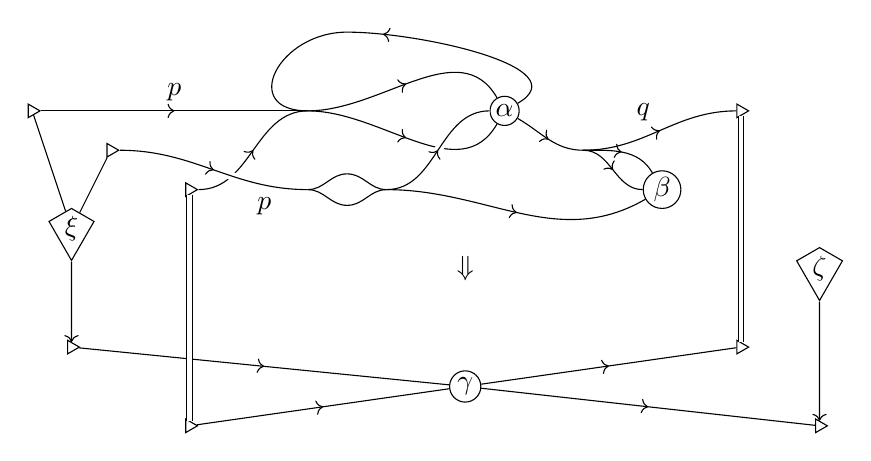
\begin{tikzpicture}
    \node[houter] (Fxy) at (.5,0) {};
    \node[houter] (idx) at (2,-1) {};
    \node[vertex] (gm) at (5.5,-.5) {$\gamma$};
    \node[houter] (idz) at (9,0) {};
    \node[houter] (G) at (10,-1) {};
    \draw[edge] (Fxy) -- (gm);
    \draw[edge] (idx) -- (gm);
    \draw[edge] (gm) -- (idz);
    \draw[edge] (gm) -- (G);
    \node[kite,draw,inner sep=1pt] (Gin) at (10,1) {$\zeta$};
    \draw[->] (Gin) -- (G);
    \node[houter] (zout) at (9,3) {};
    \draw[double,double equal sign distance] (zout) -- (idz);
    \node[houter] (xin) at (2,2) {};
    \draw[double,double equal sign distance] (xin) -- (idx);
    \node[houter] (xyinx) at (0,3) {};
    \node[houter] (xyiny) at (1,2.5) {};
    \node[kite,draw,inner sep=1pt] (F) at (.5,1.5) {$\xi$};
    \draw (xyinx) -- (F);
    \draw (xyiny) -- (F);
    \draw[->] (F) -- (Fxy);
    \node[vertex] (be) at (8,2) {$\beta$};
    \node[vertex] (al) at (6,3) {$\alpha$};
    \coordinate (x) at (3.5,3);
    \coordinate (y) at (3.5,2);
    \draw[edge] (xyinx) to[out=0,in=180] node[auto] {$p$} (x);
    \draw[edge] (xin) to[out=0,in=180] (x);
    \draw[cross] (xyiny) to[out=0,in=180] (y);
    \draw[edge] (xyiny) to[out=0,in=180] node[auto,swap,very near end] {$p$} (y);
    \draw[edge] (x) to[out=0,in=120] (al);
    \draw[edge] (x) to[out=0,in=-120] (al);
    \coordinate (y2) at (4.5,2);
    \draw[cross] (y2) to[out=0,in=-180] (al);
    \draw[edge] (y2) to[out=0,in=-180] (al);
    \draw (y) to[out=0,in=180] (4,2.2) to[out=0,in=180] (y2);
    \draw (y) to[out=0,in=180] (4,1.8) to[out=0,in=180] (y2);
    \draw[edge] (al) to[out=30,in=0] (4,4) to[out=180,in=180,looseness=2] (x);
    \coordinate (z) at (7,2.5);
    \draw[edge] (al) to[out=-30,in=180] (z);
    \draw[edge] (z) to[out=0,in=120] (be);
    \draw[edge] (z) to[out=0,in=180] (be);
    \draw[edge] (y2) to[out=0,in=-150] (be);
    \draw[edge] (z) to[out=0,in=-180] node[auto] {$q$} (zout);
    \node at (5.5,1) {$\Downarrow$};
  \end{tikzpicture}
\end{center}
would be written with the following syntax:
\begin{equation}
  x:p, y:p, z:p \mid y\doteq y \mid \alpha(x,y,x;x,z), \beta(z,z,y;) \types \gamma(\xi(x,y),x;z,\zeta).\label{eq:2cell-eg}
\end{equation}

The action of weak equivalences on mode 2-cells consists of exchange rules allowing us to permute all the contexts, together with ``reduction'' or ``substitution'' rules as in~\eqref{eq:subst}:
\begin{equation}\label{eq:reduction}
  \inferrule{\Delta,y:p\mid\Xi,x\doteq y \mid \Theta \types M \\ x\not\jdeq y}{\Delta\mid\Xi[x/y]\mid \Theta[x/y] \types M[x/y]}
  % \qquad
  % \inferrule{\Delta,x:p\mid\Xi,x\doteq y \mid \Theta \types M \\ x\not\jdeq y}{\Delta\mid\Xi[y/x]\mid \Theta[y/x] \types M[y/x]}
\end{equation}
Note that the substitution $M[x/y]$ involves substitution into the mode arrow terms appearing in $M$.
In the 1-cartesian or 2-cartesian case, we should have an action of more general hypergraph morphisms.
We saw in \cref{thm:hyctx} that these can be represented by graph context morphisms, yielding the following rule:
\begin{equation}\label{eq:hygph-action}
  \inferrule{\Delta\mid\Xi\mid\Gamma \types M
    \\ (\sigma\mid\tau\mid\nu) : (\Delta\mid\Xi\mid\Gamma) \to (\Delta'\mid\Xi'\mid\Gamma')
    \\ (\sigma\mid\tau\mid\nu)\text{ is appropriate}}
  {\Delta'\mid\Xi'\mid\Gamma' \types M[\sigma]}
\end{equation}
where the ``appropriate'' condition is empty in the 2-cartesian case, that $\nu$ is a bijection in the 1-cartesian case, and that $(\sigma\mid\tau\mid\nu)$ is a weak equivalence in the non-cartesian case.
Using the inductive characterization of weak equivalences from~\eqref{eq:weq}, the latter becomes simply a ``big-step'' version of~\eqref{eq:reduction} and its dual.

The multi-substitution rule for mode 2-cells looks like this:
\begin{equation}\label{eq:multisub}
  \inferrule{
    \Delta_i \mid \Xi_i \mid \Theta_i \types \alpha_i(\vec \xi_i)
    \\
    \Delta \mid \Xi \mid \alpha_1(\vec x_1),\dots, \alpha_n(\vec x_n) \types M
    \\
    \unifies{\Delta,\Delta_1,\dots,\Delta_n}{\Xi, \Xi_1,\dots,\Xi_n,\vec x_1 \doteq \vec \xi_1, \dots, \vec x_n \doteq \vec \xi_n}{\Phi}{\Upsilon}{\sigma}
  }
  {\Phi
    \mid
    \Upsilon
    \mid
    \Theta_1[\sigma],\dots,\Theta_n[\sigma]
    \types
    M[\sigma]}
\end{equation}
Here each $\vec x_i$ is a list of variables occurring in $\Delta$, not necessarily distinct, while each $\vec\xi_i$ is a list of mode-arrow terms in context $\Delta_i$.
I believe this really does correspond to the semantic composition operation in a virtual hypercategory.
In particular, the unification judgment checks that the inputs are well-typed and inserts the appropriate new edges coming from the graph insertions.

% In fact, I think that the extended loop contexts should also mean that we can consider only a single-entry substitution rule:
% \begin{equation}\label{eq:onevert}
%   \inferrule{
%     \Phi \mid \Upsilon \mid \Psi \types \alpha(\vec \xi)
%     \\
%     \Delta \mid \Xi \mid \Theta, \alpha(\vec x) \types M
%   }
%   {\Delta,\Phi
%     \mid
%     \Xi, \Upsilon, \vec x \doteq \vec \xi
%     \mid
%     \vec \Theta,\Phi
%     \types
%     M}
% \end{equation}
% This way we have to ``pass through junk'' in order to get to a meaningful judgment: a single substitution may yield a loop context that cannot be reduced to contain only equations between variables, yet further substitutions may add more equations making it reducible.

We also need a rule of substitution into edges that are incident to no vertices (except possibly the root)
\fxnote{Not entirely sure about the linearity of $\xi$ here (in the non-cartesian case only, of course)}
\begin{equation}\label{eq:novert}
  \inferrule{
    \Delta \types \Xi \edgectx \\
    \Delta \types \Gamma \graph \\
    \Delta',x:p \types \Xi' \edgectx\\
    \Psi \Types \xi : p \\
    \Delta,\Delta',x:p \mid \Xi,\Xi' \mid \Gamma \types M\\
    \unifies{\Delta',\Psi}{\Xi',x\doteq \xi}{\Phi}{\Upsilon}{\sigma}
  }{\Delta,\Phi \mid \Xi,\Upsilon \mid \Gamma \types M[\sigma]}
\end{equation}

We could also incorporate this as part of the multi-substitution rule~\eqref{eq:multisub}.

\begin{thm}\label{thm:mode-adm}\fxnote{I'm going to assume this is true.}
  If we represent the generating 2-cells by rules that build in~\eqref{eq:hygph-action},~\eqref{eq:multisub}, and~\eqref{eq:novert}, then these rules become admissible.
\end{thm}

In the cartesian cases, probably we can build~\eqref{eq:hygph-action} into the variable rule in a way that looks more like usual cartesian type theory.

This completes the first description of a type theory for virtual hypercategories.
Now we reorganize it to make it look different.
I will discuss this only in the non-cartesian case, since it is simpler and I think it is the one of most interest for this presentation.

Recall that in traditional natural deduction, a hypothetical judgment such as $A,B\types C$ is (or at least, can be regarded as being) introduced as a shorthand for a derivation tree of $C$ that retains $A$ and $B$ as hypothesis leaves.
That is, instead of writing
\[ \inferrule{
  {\begin{array}{c}
    A \\ \vdots
  \end{array}}
  \\
  {\begin{array}{c}
    B \\ \vdots
  \end{array}}}{C} \]
and remembering that $A$ and $B$ were hypotheses in the derivation of $C$, we keep a list of all current hypotheses in the context at each node of the derivation tree:
\[ \inferrule{
  {\begin{array}{c}
    \inferrule{ }{A\types A} \\ \vdots
  \end{array}}
  \\
  {\begin{array}{c}
    \inferrule{ }{B\types B} \\ \vdots
  \end{array}}}{A,B\types C} \]
One might say this is responsible for the characteristic feature of natural deduction theories when expressed in the $\Gamma\types C$ form, namely that the conclusion always has an arbitrary context $\Gamma$.

What we are going to do now is pass \emph{backwards} along a similar equivalence, starting with the above-described type theory for virtual hypercategories.
We will \emph{remove} the edge variables, loop equalities, and graph vertices from the context, placing them instead at leaves of the derivation tree.

We also change the notation a bit.
We will refer to the variables in an edge context as \emph{types} (or, more precisely, \emph{type metavariables}), and write their corresponding leaf hypotheses as
\[ A \type_p \]
instead of $A:p$.
We write each generating mode arrow $\omega : (p_1,\dots,p_n) \to q$ as a \emph{type formation rule}
\[ \inferrule{A_1 \type_{p_1}\\ \cdots \\ A_n \type_{p_n}}{\form{\omega}(A_1,\dots,A_n)} \]
The fact that the type theory for arrow terms $\Delta\types \xi:p$ is formulated in natural-deduction style means that we can represent any such term essentially uniquely as a derivation tree of type formation rules.
For instance, the term
\[x:p, y:q \types \omega(x,\varpi(y,x)) : s\]
corresponds to the tree
\[
\inferrule*{A\type_p \\ \inferrule*{B\type_q \\ A\type_p}{\form\varpi(B,A)\type_r}}{\form\omega(A,\form\varpi(B,A))\type_s}
\]
If we need the linear version $\Delta\Types \xi :p$, we can stipulate that no type metavariable occurs more than once as a hypothesis.

The equalities in the loop context we write unsurprisingly as $A\doteq B$.
Note that these are never the conclusion of a rule; they appear only as hypotheses.

We will refer to a vertex $A_1:p_1, \dots ,A_n:p_n \types \alpha(A_1,\dots,A_n) \vertex$ as a \emph{sequent} and write it
\[ \types_\alpha A_1,\dots,A_n \]
In the directed case, the entries $A_i$ separate into a domain and codomain, and we write the sequent instead as
\[ A_1\dots,A_n \types_\alpha B_1,\dots,B_m\]
Sequents can appear as both hypotheses and conclusions, but when they appear as hypotheses all the types in them must be metavariables, whereas when they appear as conclusions the types can also involve type formers.
(Thus, we are describing something that looks somewhat like a sequent calculus.)

Finally, each generating 2-cell, expressed as in \cref{thm:mode-adm} with substitutions built in, yields a derivation rule for such sequents.
I'm not sure exactly how to state this formally in general, but the idea is that given a generating 2-cell
\[ \Delta \mid \Xi \mid \alpha_1(\vec x_1),\dots, \alpha_n(\vec x_n) \types M \]
the corresponding derivation rule is obtained as follows:
\begin{itemize}
\item There is one premise of the form $\types_{\alpha_i} A_{i1},\dots,A_{i m_i}$ for each $1\le i\le n$.
\item There is one premise of the form $B_j\type_{q_j}$ for each $\Xi$-connected component in $\Delta$ that $\Xi$ does not equate to any variable appearing in any $\alpha_i$.
\item There is a type equality premise for each equality in $\Xi$.
\item There is a side condition of unification that can produce more type equalities.
\end{itemize}
To apply such a rule in the course of constructing a derivation, we assume that we have constructed derivations of $\types_{\alpha_i} A_{i1},\dots,A_{i m_i}$ for some types $A_{i k}$ (not necessarily metavariables, they may involve type formers), and similarly of $B_j \type_{q_j}$ for some types $B_j$.
We stipulate that each of these derivations must have disjoint hypotheses.
We then have to perform the unification steps from~\eqref{eq:multisub} and~\eqref{eq:novert}, using the information about coincidence of variables in the $\vec x_i$'s to produce new type equalities that also appear as premises (new hypotheses).

Finally, we can reduce away as many type equalities (between distinct type metavariables) as we want.
In general, we can describe this in a ``canceled hypothesis'' style by crossing out the equality being reduced and similarly crossing out and replacing the sequents in which the substitution must be performed.
For instance, reducing the equality $A\doteq B$ on the right in the following derivation:
\begin{equation}
\inferrule*{\types_\alpha A \\ A\doteq B \\
\inferrule*{B\types_\beta B \\ C\type_q}{B\types_\gamma \form\varpi(C)}}{\types_\delta B, \form\omega(A),\form\varpi(C)}\label{eq:unreduced-eg}
\end{equation}
yields the following
\[
\inferrule*{{\types_\alpha A} \\ \cancel{A\doteq B} \\
\inferrule*{
  \inferrule*{}{
      A\types_\beta A \\\\
      \cancel{B\types_\beta B}}
    \\ C\type_q}{B\types_\gamma \form\varpi(C)}}{
  \inferrule{}{
    \cancel{\types_\delta B, \form\omega(A),\form\varpi(C)} \\\\
    \types_\delta A, \form\omega(A),\form\varpi(C)
  }}
\]
Usually, however, for any given generating 2-cell there will be only a few equalities that can be reduced in a canonical way, and so we don't need to notate this step explicitly; in the above example we can simply write
\[
\inferrule*{{\types_\alpha A} \\ 
\inferrule*{A\types_\beta A \\ C\type_q}{A\types_\gamma \form\varpi(C)}}{\types_\delta A, \form\omega(A),\form\varpi(C)}
\]
Formally, the type theory for virtual hypercategories also includes the derivation~\eqref{eq:unreduced-eg} without any reduction.
However, in most cases it should be possible to ignore this.

By reformulating the type theory of virtual hypercategories in this way, we see that it now looks like a sequent calculus for an ``object language'', where the \emph{generating arrows and 2-cells} of the virtual hypercategory correspond to \emph{type formation and sequent deduction rules} in the object language.
Put differently, the mode theory behaves like a ``logical framework'' for the type theory.
The object-language judgments such as $A\type_p$ and $\Gamma\types_\alpha \Delta$ are represented by two kinds of ``types'' in the mode theory, which we actually call ``modes'' and ``mode morphisms'' respectively.
Similarly, the object-language rules are represented by entailments in the mode theory: mode multi-arrows and 2-cells.
Unlike an ordinary logical framework, a mode theory is very restricted in the kind of type dependency it allows --- mode morphisms can depend on modes, but that is all --- but the principle of the representation is analogous.
(In fact, this restrictiveness is actually the whole point, in accord with the ``power of weak frameworks'' philosophy of LF: by restricting what we can say in the framework, we can prove more metatheorems about it.
In our case, we can hopefully prove a fairly general cut-elimination theorem for these object-language sequent calculi.)


\section{Type-theoretic examples}
\label{sec:examples}

For now, we consider only examples without type formation rules, so that our virtual hypercategories have only identity multi-arrows.
We begin with directed examples, which are more familiar.

For the moment, we consider only the ``local picture'', i.e.\ how the derivation rules arising from specific generating 2-cells correspond to the structural rules of various well-known type theories.
Later on we will consier global questions such as semantics and initiality.


\subsection{Ordered logic}
\label{sec:ordered-logic}

We have one mode $p$, and one mode morphism $\alpha_n(\overbrace{p,p,\dots,p}^n;p)$ for each $n$.
The 2-cells are generated by the identity and composition
\begin{mathpar}
  x:p \mid \cdot \mid \cdot \types \alpha_1(x,x)
  \and
  \Delta,\Phi_1,\Phi_2,y:p,z:p \mid\cdot \mid \alpha_n(\Delta;y), \alpha_{k+1+m}(\Phi_1,y,\Phi_2;z)
  \types \alpha_{k+n+m}(\Phi_1,\Delta,\Phi_2;z)
  % x_1:p,\dots,x_n:p,z:p,y_1:p,\dots,y_m:p \mid \cdot \mid u:\alpha_n(\vec x;y_i), v:\alpha_m(\vec y;z) \\
  % \types v\circ_i u : \alpha_{n+m-1}(y_1,\dots,y_{i-1},x_1,\dots,x_n,y_{i+1},\dots,y_m;z)
\end{mathpar}
We also impose the axioms of a multicategory, as presented in the ``one-place composition'' style.
Note that the order of the edge and vertex variables doesn't matter, since we always have exchange for those; what imposes the ordering on the object logic is the order of arguments to the $\alpha_n$'s.

These generating 2-cells yield the identity and cut rules for the corresponding type theory:
\begin{mathpar}
  \inferrule{A\type_p}{A\types_{\alpha_1} A}
  \and
  \inferrule{\Gamma\types_{\alpha_n} B \\ B\doteq C \\ \Psi_1,C,\Psi_2 \types_{\alpha_{k+1+m}} D}
  {\Psi_1,\Gamma,\Psi_2\types_{\alpha_{k+n+m}} D}
\end{mathpar}
Since there is exactly one mode morphism of each arity, the subscript of $\types_{\alpha_n}$ is uniquely determined by the number of types on the left, so we can omit it.
Similarly, we can omit the subscript on $A\type_p$ since there is only one mode.
If we additionally perform the obvious equality reduction in the cut rule, we obtain exactly the usual rules for ordered logic:
\begin{mathpar}
  \inferrule{A\type}{A\types A}
  \and
  \inferrule{\Gamma\types B \\ \Psi_1,B,\Psi_2 \types D}
  {\Psi_1,\Gamma,\Psi_2\types D}
\end{mathpar}

If we wanted, we could instead use 2-cells generating multi-composition:
\begin{multline*}
  \Phi_1,\dots,\Phi_m,y_1:p,\dots,y_m:p,z:p \mid\cdot\mid\\
  \alpha_{n_1}(\Phi_1;y_1),\dots,\alpha_{n_m}(\Phi_m;y_m), \alpha_m(y_1,\dots,y_m;z)\\
  \types \alpha_{n_1+\cdots+n_m}(\Phi_1,\dots,\Phi_m;z)
\end{multline*}
with the appropriate axioms.
The equivalence between the two definitions of multicategory can then be phrased as an isomorphism between the virtual hypercategories having these two presentations.

In this case, as in some others, the virtual hypercategory presented by these generators and relations can be described directly in a global way: there is exactly one 2-cell whose domain is any \emph{planar directed tree}.
This amounts to a coherence theorem for multicategories.


\subsection{Intuitionistic linear logic}
\label{sec:ill}

To ordered logic we add a symmetry 2-cell
\[ \Delta,x:p,y:p,\Phi,z:p \mid\cdot \mid \alpha_n(\Delta,x,y,\Phi;z) \types \alpha_n(\Delta,y,x,\Phi;z) \]
generating the exchange rule:
\[ \inferrule{\Gamma,A,B,\Psi \types C}{\Gamma,B,A,\Psi \types C} \]
together with axioms on its composites and relating it to the composition operations, as in the definition of symmetric multicategory.
Note that with only one sequent premise, the unification step is trivial and no type equalities are generated.

We could instead add an unbiased exchange rule for any permutation $\sigma$:
\[ \Delta,z:p \mid\cdot \mid \alpha_n(\Delta;z) \types \alpha_n(\Delta^\sigma;z) \]
and prove that it generates an isomorphic mode theory.

The corresponding coherence theorem involves \emph{non-planar} directed trees.


\subsection{Intuitionistic nonlinear logic}
\label{sec:intu-nonl-logic}

Similarly, we can add contraction and weakening 2-cells:
\begin{mathpar}
  \Delta,x:p,z:p \mid\cdot \mid \alpha_{n+2}(\Delta,x,x;z) \types  \alpha_{n+1}(\Delta,x;z)
  \and
  \Delta,x:p,z:p \mid\cdot \mid \alpha_n(\Delta;z) \types \alpha_{n+1}(\Delta,x;z)
\end{mathpar}
generating the usual rules:
\begin{mathpar}
  \inferrule{\Gamma,A,A\types C}{\Gamma,A\types C}
  \and
  \inferrule{A\type \\ \Gamma\types C}{\Gamma,A\types C}.
\end{mathpar}
Note that every distinct type metavariable appearing in a premise or a conclusion of the rule corresponds to exactly one edge variable in the mode 2-cell.
We impose the axioms of a cartesian multicategory.

Of course we could also use 2-cells parametrized by arbitrary functions of finite sets.
But I don't know a description of the entire mode theory analogous to the directed trees used in the linear case.


\subsection{Classical linear logic}
\label{sec:cll}

Still with only one mode $p$, suppose instead we have mode morphisms
\[\alpha_{n,m}(\overbrace{p,\dots,p}^n,\overbrace{p,\dots,p}^m)\]
for each $n,m$.
As before, since there is a unique mode morphism with each directed arity, we can omit the label on sequents without ambiguity.

We have symmetry 2-cells on both sides
\begin{mathpar}
\Delta,x:p,y:p,\Phi,\Theta \mid\cdot \mid \alpha_{n,m}(\Delta,x,y,\Phi;\Theta) \types \alpha_{n,m}(\Delta,y,x,\Phi;\Theta)
\and
\Delta,x:p,y:p,\Phi,\Theta \mid\cdot \mid \alpha_{n,m}(\Delta;\Theta,x,y,\Phi) \types \alpha_{n,m}(\Delta;\Theta,y,x,\Phi)
\end{mathpar}
generating the exchange rules:
\begin{mathpar}
\inferrule{\Gamma,A,B,\Psi \types \Theta}{\Gamma,B,A,\Psi \types \Theta}
\and
\inferrule{\Gamma \types \Theta,A,B,\Psi}{\Gamma \types \Theta,B,A,\Psi}
\end{mathpar}
The same identity 2-cell
\[ x:p \mid \cdot \mid \cdot \types \alpha_1(x,x) \]
generates the identity rule
\[ \inferrule{ }{A\types A}\]
And the following family of 2-cells
\[ \Delta,\Theta,x:p,\Gamma,\Psi \mid\cdot\mid \alpha_{n,m+1}(\Delta;\Theta,x), \alpha_{1+k,\ell}(x,\Gamma;\Psi) \types \alpha_{n+k,m+\ell}(\Delta,\Gamma;\Theta,\Psi) \]
generates a cut rule with type equality
\[ \inferrule{\Delta \types \Theta,A \\ A\doteq B \\ B,\Gamma \types \Psi}{\Delta,\Gamma \types \Theta,\Psi} \]
that reduces canonically to the usual cut rule of linear logic:
\[ \inferrule{\Delta \types \Theta,A \\ A,\Gamma \types \Psi}{\Delta,\Gamma \types \Theta,\Psi} \]
We impose the usual axioms of a symmetric polycategory~\cite{szabo:polycats}, also known as a (colored) dioperad~\cite{gan:dioperads}.
There is also a ``multi-composition'' definition of polycategory~\cite{koslowski:polycats,garner:polycats}, and the coherence theorem involves all directed (binary) graphs that are undirected trees.


\subsection{Classical nonlinear logic}
\label{sec:cl}



\subsection{Props and their cousins}
\label{sec:props}




\subsection{Flavors of operad}
\label{sec:operads}

All of these use only binary directed graphs.
A summary is in~\cite{bb:htapm}.

Directed sorts:
\begin{itemize}
\item Wheeled props~\cite{mms:wheeled-props} use arbitrary directed graphs.
\item Props use directed graphs with no directed loops.
\item Properads~\cite{vallette:properads} use connected directed graphs with no directed loops.
\item Wheeled properads use arbitrary connected directed graphs.
\item Dioperads~\cite{gan:dioperads} / polycategories~\cite{szabo:polycats,koslowski:polycats,garner:polycats} have no directed loops and are connected and simply connected (no undirected loops either), or equivalently contractible.~\cite{markl:operads-props}
% \item Symmetric operads/multicategories use arbitrary directed trees.
% \item Non-symmetric operads/multicategories use planar directed trees.
\item Compact closed categories~\cite{kl:cpt}.
\end{itemize}

Undirected sorts:
\begin{itemize}
\item Cyclic operads~\cite{gk:cyclic-operads} use undirected trees; compare to~\cite{co:flang-cyclic,co:cat-cyclic}.
\item Modular operads~\cite{gk:modular-operads} use arbitrary connected graphs (plus a ``stability'' condition).
\item Compact symmetric multicategories~\cite{jk:feynman} use arbitrary graphs.
  This is a somewhat misleading name as it doesn't indicate that the objects are actually \emph{self-}dual (the undirectedness).
\end{itemize}

All of these can be categorified (or virtualized) by considering non-discrete opfibrations (resp.\ just maps) of virtual hypercategories.
In the case of compact closed categories, the virtualized result is kits; so a kit is really literally a ``virtual compact closed double category'' in this sense.


\bibliography{../all.bib}
\bibliographystyle{alpha}

\end{document}
